%!TEX root = ../my_thesis.tex

\graphicspath{{main/chapter2/fig/}}

\chapter{Efficient Algorithms for Digital Communication Receivers}
\label{chap:alg}

The purpose of this chapter is to describe different receiver algorithms and
methods representative of today and future digital communication standards.
% The optimized algorithms implementations will be discussed in the next chapter.
The first section of this chapter defines the mathematical operators used in the
other sections.

The second section presents the LDPC codes, first the encoding scheme is
detailed and then the Belief Propagation decoder and its variants are detailed
and compared.

The third section presents the polar codes, first the encoding scheme is
detailed and then the most famous decoding algorithms are explained and
compared.
% The notion of genericity and decoder flexibility are defined.

The fourth section presents the Turbo codes encoding scheme as well as the turbo
decoding algorithm. The BCJR sub-encoder and its variants are presented and
compared.

The fifth section presents the sparse code multiple access mechanism. The
encoding and decoding schemes are presented and a new algorithmic approximation
of the message passing algorithm is proposed and evaluated in terms of
error-rate performance.

\vspace*{\fill}
\minitoccustom
\vspace*{\fill}

\section{Prerequisites}

\begin{table}[htp]
  \centering
  \caption{Elementary operations in $GF_2$ (logical \emph{exclusive or} and
    \emph{and}).}
  \label{tab:alg_gf2_operations}
   \begin{tabular}{c c c c}
   $a$ & $b$ & $a \oplus b$ & $ab$ \\
    \hline
    \hline
    0 & 0 & 0 & 0 \\
    0 & 1 & 1 & 0 \\
    1 & 0 & 1 & 0 \\
    1 & 1 & 0 & 1 \\
  \end{tabular}
\end{table}

In all the presented coding schemes, only binary codes are considered. In this
case, a bit can be represented in a Galois field of two elements $\{0, 1\}$
denoted as $GF_2$. A block code is an application $g$ of $GF_2^K$ in $GF_2^N$
with $K < N$. There are $2^K$ codewords $\bm{c}$. The two operators used to
generate a codeword are the addition and the multiplication. In $GF_2$, the
addition is equivalent to the logical \emph{exclusive or} ($\oplus$) and
the multiplication is equivalent to the logical \emph{and} (cf.
Table~\ref{tab:alg_gf2_operations}).

In this section, all the presented decoders are working on \emph{soft}
information. This mean that the decoders input is a vector of $N$ likelihoods in
the form of LLRs. Each LLR is a real value. Depending on the implementation it
can be a floating-point or a fixed-point number. It results in more complex
operations than for the encoding process. On the decoder side and in the
logarithmic domain, the $\oplus$ operator becomes the $\boxplus$ operator, it is
defined as follow:
\begin{equation}
  l_a \boxplus l_b = 2\tanh^{-1}{\big(\tanh{(\frac{l_a}{2}).\tanh{(\frac{l_b}{2})}}\big)}.
\end{equation}
This is the main reason why, in channel coding, the decoders are systematically
more compute intensive than the encoders. In the logarithmic domain, the
multiplication becomes a simple addition.

\section{Low-Density Parity-Check Codes}
\label{sec:alg_ldpc}

\subsection{Coding Scheme}

A parity-check constraint is an equation that links a set of bits: when all the
bits of a parity-check constraint are added together the result has to be
zero. For instance, if we consider a message $\bm{u} = [u_0, u_1, u_2, u_3]$
($K = 4$). It is possible to encode the information message $\bm{u}$ in a
codeword $\bm{c}$ of size $N = K + 1 = 5$: $\bm{c} = [u_0,u_1,u_2,u_3,p_0]$.
The parity-check constraint $\mathcal{C}_0$ is then: $u_0 \oplus u_1 \oplus u_2
\oplus u_3 \oplus p_0 = 0~(\mathcal{C}_0)$ with $p_0$ the parity bit ($P = N -
K = 1)$. To encode the message $\bm{u}$ and produce the codeword $\bm{c}$, a
generator matrix $\bm{\mathcal{G}}$ (or a linear application) can be defined
like this: $\bm{c} = \bm{u} \times \bm{\mathcal{G}}$ with
\begin{equation*}
\bm{\mathcal{G}} =
\begin{bmatrix}
1 & 0 & 0 & 0 & 1\\
0 & 1 & 0 & 0 & 1\\
0 & 0 & 1 & 0 & 1\\
0 & 0 & 0 & 1 & 1\\
\end{bmatrix}
.
\end{equation*}
$\bm{u} \times \bm{\mathcal{G}} = [u_0,u_1,u_2,u_3,u_0 \oplus u_1 \oplus u_2
\oplus u_3] = \bm{c}$, so $p_0 = u_0 \oplus u_1 \oplus u_2 \oplus u_3$ as
defined by the parity-check constraint $\mathcal{C}_0$. The proposed
$\bm{\mathcal{G}}$ generator matrix is composed by the identity matrix on the
four first columns and by the parity-check constraint in the last column.
The consequence of the presence of the identity matrix is that the generated
codeword contains the initial information bits $u_0$, $u_1$, $u_2$, and $u_3$.
In this case, the encoding process is called \emph{systematic}.

\begin{figure}[htp]
  \centering
  \includegraphics{ldpc/parity_check/parity_check}
  \caption{Representation of the $\mathcal{C}_0$ parity-check constraint on a
    Tanner graph.}
  \label{fig:alg_ldpc_parity_check}
\end{figure}

One can note that a parity-check constraint can also be represented with a
Tanner graph (or a bipartite graph) as shown in
Fig.~\ref{fig:alg_ldpc_parity_check}. It is also possible to define a matrix of
parity-check constraints namely $\bm{\mathcal{H}}$. In the present case, there
is only one constraint ($\mathcal{C}_0$), so $\bm{\mathcal{H}}$ is a
one-dimension matrix (or a vector) of size $N$:
$
\bm{\mathcal{H}} =
\begin{bmatrix}
1 & 1 & 1 & 1 & 1
\end{bmatrix}.
$
An important property of the $\bm{\mathcal{H}}$ matrix is that it must satisfy:
$\bm{\mathcal{G}} \times \bm{\mathcal{H}}^T = \bm{0}.$

\begin{figure}[htp]
  \centering
  \includegraphics{ldpc/parity_checks/parity_checks}
  \caption{Parity-check constraints of an LDPC code on a Tanner graph.}
  \label{fig:alg_ldpc_parity_checks}
\end{figure}

The construction of an Low-Density Parity-Check (LDPC) code is based on the
combination of many parity-check nodes. Fig.~\ref{fig:alg_ldpc_parity_checks} is
an example of LDPC code with four parity-check constraints denoted as $a$, $b$,
$c$ and $d$. The parity-check constraints are also known as the \emph{check
nodes} ($C_N$). And the \emph{variable nodes} ($V_N$) are the bits of the LDPC
codeword. The parity-check matrix corresponding to the
Fig.~\ref{fig:alg_ldpc_parity_checks} Tanner graph is:
\begin{equation*}
\bm{\mathcal{H}} =
\begin{bmatrix}
  1 & 0 & 0 & 1 & 1 & 0 & 1 & 1\\
  0 & 1 & 1 & 0 & 0 & 1 & 1 & 0\\
  1 & 0 & 1 & 0 & 0 & 1 & 0 & 1\\
  0 & 1 & 0 & 1 & 1 & 0 & 1 & 0
\end{bmatrix}.
\end{equation*}

The $\bm{\mathcal{H}}$ parity matrix of an LDPC code has to be a low-density
matrix (less that 3\% of 1). The example shown in
Fig.~\ref{fig:alg_ldpc_parity_checks} is here to help to the comprehension and
is not a real LDPC code: there is much more than 3\% of 1 in the corresponding
$\bm{\mathcal{H}}$ matrix.

\subsection{Belief Propagation Decoding Algorithm}

The bit $\hat{u}_n$ corresponding to the input LLR $l_n$ of a parity-check code
can be decoded as follow: $\hat{u}_n = \hardDec\big(l_n +
\sum\limits_{j \neq n}{l_j}\big)$, with $\hardDec$ the hard decision function
that returns 0 if the LLR is positive and 1 else. For instance, considering the
parity-check code in Fig.~\ref{fig:alg_ldpc_parity_check}, $\hat{u}_0 =
\hardDec\big(l_0 + (l_1 \boxplus l_2 \boxplus l_3 \boxplus l_4)\big)$,
$\hat{u}_1 = \hardDec\big(l_1 + (l_0 \boxplus l_2 \boxplus l_3 \boxplus
l_4)\big)$, etc.

In LDPC codes, there is more than one parity-check node, it is then possible to
compute all the check nodes connected to a variable node and to store the result
in vector $\bm{v}$. Each LLR $v_n \in \bm{v}$ corresponds to a variable node.
For instance, considering Fig.~\ref{fig:alg_ldpc_parity_checks}, $V_0$ is
connected to $C_a$ and $C_c$ so its LLR value can be computed as follow: $v_0
= e_0 + e_1 = (l_3 \boxplus l_4 \boxplus l_6 \boxplus l_7) + (l_2 \boxplus l_5
\boxplus l_7)$, where $e_0$ and $e_1$ are the extrinsic information computed
respectively from $C_a$ and $C_c$. The decoded bits can be decided from the
channel and the variable node LLR values: $\hat{u}_n = \hardDec{(l_n + v_n)}$.

In the Belief Propagation (BP) decoding algorithm, there are many iterations (5
to 100) between the variable nodes and the check nodes, before to decide the
decoded bits $\bm{\hat{u}}$. In the first iteration, the a priori information
$\bm{a}$ sent to the check nodes is directly the channel values $\bm{l}$. But,
in the next iterations, the a priori information $\bm{a}$ is updated with the
variable nodes values $\bm{v}$. To avoid direct auto-confirmation issues, the
up-coming extrinsic LLR is systematically subtracted to the propagated message.

\begin{figure}[htp]
  \centering
  \subfloat[][Check nodes update.]
  {
    \includegraphics[scale=0.9]{ldpc/bp_cn_update/bp_cn_update}
    \label{fig:alg_ldpc_bp_cn_update}
  }
  \quad
  \subfloat[][Variable nodes update.]
  {
    \includegraphics[scale=0.9]{ldpc/bp_vn_update/bp_vn_update}
    \label{fig:alg_ldpc_bp_vn_update}
  }
  \caption{Illustration of the belief propagation algorithm on a Tanner graph.}
  \label{fig:alg_ldpc_bp}
\end{figure}

Fig.~\ref{fig:alg_ldpc_bp} illustrates a single BP iteration. First, the check
nodes are computed from the messages $m_j^i$ where $i$ is the index of the
variable nodes and $j$ is the index of the check nodes. In the example, the
$C_a$ check node computes $a^0_a \boxplus a^3_a \boxplus a^4_a \boxplus a^6_a
\boxplus a^7_a$, where $a^0_a = l_0 + v_0 - e^{0}_a$, $a^3_a = l_3 + v_3 -
e^{3}_a$, etc. In the first iteration $\bm{v}$ and $\bm{e}$ are initialized to
0. Then, when all the check nodes have been computed it is possible to
determine the new values of the $v_n$ variable nodes from the sum of the
incoming extrinsic messages $e_j^n$. In the example, $v_0 = e^0_a + e^0_c$,
where $e^0_a = a^3_a \boxplus a^4_a \boxplus a^6_a \boxplus a^7_a$ and $e^0_c =
a^2_c \boxplus a^5_c \boxplus m^7_c$. When all the variable nodes have been
updated, it is then possible to update the check nodes and so on.

\begin{figure}[htp]
  \centering
  \includegraphics[width=0.7\textwidth]{ldpc/iterations/iterations}
  \caption
    [Decoding performance of the BP algorithm depending on the iterations.]
    {Decoding performance of the belief propagation algorithm depending on the
     number of iterations. IEEE 802.16e (WiMAX) $\mathcal{H}$ parity matrix
     ($N=2304$, $R=1/2$).}
  \label{plot:alg_ldpc_iterations}
\end{figure}

Fig.~\ref{plot:alg_ldpc_iterations} shows the decoding performance of the BP
algorithm depending on the number of iterations. Each time the number of
iterations is doubled (from 5 to 40). A $\mathcal{H}$ parity matrix from the
WiMAX standard (IEEE 802.16e) is used. The need to perform many BP decoding
iterations is demonstrated. The computational effort required by the BP decoder
increases with the number of iterations. Thus, depending on the constraint
(latency, throughput, correction power, etc.) the system designer can choose an
appropriate number of iterations. The required decoding computational effort can
be reduced by implementing an early termination criterion. At the end of an
iteration it is possible to decide the $\bm{\hat{u}}$ bits and to check if these
bits verify the parity check constraints of the $\bm{\mathcal{H}}$ matrix. If
yes, the decoder can stop before performing all the iterations. This is also
called the syndrome verification.

There are many variants of the BP algorithm, in the previous explanation, in an
iteration, all the check nodes are computed first and then all the variable
nodes are updated. This is what we call a \emph{flooding} (BP-F) scheduling of
the computations~\cite{MacKay1995}. However it is possible to schedule the
computations differently. In the \emph{horizontal layered} (BP-HL)
scheduling~\cite{Yeo2001}, when a check node is evaluated, all the connected
variable nodes are updated without waiting the computation of all the check
nodes. In the \emph{vertical layered} (BP-VL) scheduling~\cite{Zhang2002}, the
check nodes corresponding to a variable node are evaluated and the current
variable node is updated. The vertical layered scheduling traverses the variable
nodes first while the horizontal layered scheduling processes the check nodes
first. In general, the layered scheduling (vertical and horizontal) allows to
converge faster (in less iterations than the flooding) to a valid codeword.

\begin{figure}[htp]
  \centering
  \includegraphics[width=0.7\textwidth]{ldpc/scheduling/scheduling}
  \caption
    [Decoding performance of the BP algorithm depending on the scheduling.]
    {Decoding performance of the belief propagation algorithm depending on the
     scheduling. Flooding (BP-F), horizontal layered (BP-HL) and vertical
     layered (BP-VL) scheduling are considered. IEEE 802.16e (WiMAX)
     $\mathcal{H}$ parity matrix ($N=2304$, $R=1/2$).}
  \label{plot:alg_ldpc_scheduling}
\end{figure}

Fig.~\ref{plot:alg_ldpc_scheduling} shows the decoding performance depending on
the scheduling. The horizontal and vertical layered scheduling have
approximatively the same level of performance. The decoding performance of the
layered scheduling is more interesting than the flooding scheduling. Thus, one
decoding iteration with the layered scheduling is approximatively equal to two
flooding iterations.

In the previous example, the rules to update the variable nodes are based on the
$\boxplus$ operator. In the literature, this type of update rules is called the
\emph{Sum-Product Algorithm} (SPA) and was first introduced by Gallager in
1962~\cite{Gallager1962}. The SPA results in very good BER/FER decoding
performance. However, this comes at the cost of a high computational complexity.
To reduce the complexity on the $\boxplus$ operator it is possible to
approximate it as follow:
\begin{equation}
\label{eq:alg_ldpc_ms}
l_a \boxplus l_b = 2\tanh^{-1}{\big(\tanh{(\frac{l_a}{2}).\tanh{(\frac{l_b}{2})}}\big)} \approx \sign(l_a.l_b).\min(|l_a|, |l_b|).
\end{equation}
This variant is called the \emph{Min-Sum} (MS)~\cite{Fossorier1999}.
The expensive $\tanh$ functions are replaced by efficient $\sign$ and $\min$
operators. However, MS computations negatively affect the correction
performance. To solve this issue, the optimized \emph{Offset Min-Sum} (OMS) and
\emph{Normalized Min-Sum} (NMS) approximations have been proposed
in~\cite{Chen2002}:
\begin{equation}
\label{eq:alg_ldpc_onms}
l_a \boxplus l_b = 2\tanh^{-1}{\big(\tanh{(\frac{l_a}{2}).\tanh{(\frac{l_b}{2})}}\big)} \approx \alpha \times \big( \sign(l_a.l_b).\min(|l_a|, |l_b|) + \lambda \big),
\end{equation}
where $\alpha$ is the normalization factor of the NMS update rules and $\lambda$
is the offset of the OMS update rules.

\begin{figure}[htp]
  \centering
  \includegraphics[width=0.7\textwidth]{ldpc/update_rules/update_rules}
  \caption
    [Decoding performance of the BP algorithm depending on the update rules.]
    {Decoding performance of the belief propagation algorithm depending on the
     update rules (horizontal layered scheduling). 40 iterations, IEEE 802.16e
     (WiMAX) $\mathcal{H}$ parity matrix ($N=2304$, $R=1/2$).}
  \label{plot:alg_ldpc_update_rules}
\end{figure}

Fig.~\ref{plot:alg_ldpc_update_rules} shows the decoding performance of the
belief propagation algorithm depending on the update rules presented before.
As expected, there is a significant performance degradation with the MS
approximation. The OMS and NMS update rules are very close to the SPA. These
results demonstrate the efficiency of the OMS and NMS approximations. In real
systems they are very often preferred to the original SPA.

\section{Polar Codes}
\label{sec:alg_polar}

\subsection{Coding Scheme}

A polar code $(N,K)$ is a linear block code of size $N = 2^m$, with $N$ the
first natural number higher than $K$. The $\bm{\mathcal{G}}$ generator matrix of
a polar code can recursively be defined by the $m^\text{th}$ Kronecker power of
$\bm{\mathcal{K}} =
\begin{bmatrix}
1 & 0 \\
1 & 1
\end{bmatrix},$
denoted as
$
\bm{\mathcal{G}} = \bm{\mathcal{K}}^{\otimes m} =
\begin{bmatrix}
\bm{\mathcal{K}}^{\otimes m-1} & 0_{m -1} \\
\bm{\mathcal{K}}^{\otimes m-1} & \bm{\mathcal{K}}^{\otimes m-1}
\end{bmatrix},
$
composed by $N$ lines and $N$ columns. Unlike for the LDPC codes, the $\bm{u}$
input message cannot be directly multiplied by $\bm{\mathcal{G}}$ because
$\bm{\mathcal{G}}$ is a square matrix of dimension $N$. So, the polar coding
scheme defines a $\mathcal{F}$ function that adds zeros in $\bm{u}$ until its
size reaches $N$ bits ($\bm{v} = \mathcal{F}(\bm{u})$). If we suppose a $(8,4)$
polar code, $\bm{u} = [u_0, u_1, u_2, u_3]$ is composed of 4 information bits.
Lets apply the $\mathcal{F}$ function on $\bm{u}$: $\mathcal{F}(\bm{u}) =
[0, 0, 0, u_0, 0, u_1, u_2, u_3] = \bm{v}$. There is $N$ output bits in
$\bm{v}$. The extra zeros are called the \emph{frozen bits}, their positions in
$\bm{v}$ are selected to be on the less reliable indexes. In other terms, the
information bits occupy the most reliable positions in $\bm{v}$. The frozen bits
represent the $P$ parity bits. In this thesis, the Gaussian Approximation (GA)
method is used to determine the position of the frozen bits~\cite{Trifonov2012}.
To summarize, the polar encoding process can be defined as follow: $\bm{c} =
\mathcal{F}(\bm{u}) \times \bm{\mathcal{G}} = \bm{v} \times \bm{\mathcal{G}}$.

\begin{figure}[htp]
  \centering
  \includegraphics[width=1.0\linewidth]{polar/encoder/encoder}
  \caption{Polar encoders for $N \in \{2, 4, 8\}$ and $R = 1/2$.}
  \label{fig:alg_polar_encoder}
\end{figure}

Fig.~\ref{fig:alg_polar_encoder} presents $\bm{\mathcal{G}}$ generator
matrices depending on $N$ and their associate encoding schemes described with
factor graphs. The recursive structure of the polar codes is represented by the
dashed rectangles in the factor graphs. For instance, when $N = 8$, the encoder
is composed of two $N = 4$ sub-encoders and each $N = 4$ sub-encoder is itself
composed of two $N = 2$ sub-encoders. The polar code are not necessarily
systematic. In fact, the encoding process is only systematic when there is a
unique information bit ($K =1$).

\begin{figure}[htp]
  \centering
  \includegraphics[scale=1.0]{polar/encoder_sys/encoder_sys}
  \caption{Systematic polar encoder for $N = 8$ and $R = 1/2$.}
  \label{fig:alg_polar_encoder_sys}
\end{figure}

In 2011, \Arikan proposed a systematic coding scheme for the polar
codes~\cite{Arikan2011}. The idea is to encode $\bm{u}$ two times instead of
one. Fig.~\ref{fig:alg_polar_encoder_sys} shows the systematic polar
encoder for $N = 8$. The systematic encoding scheme can be expressed as:
$\bm{c} = \mathcal{F'}\big(\mathcal{F}(u) \times \bm{\mathcal{G}}\big) \times
\bm{\mathcal{G}}$, with $\mathcal{F'}$ the function that reinitializes the
frozen bits to zero after the first encoding. The systematic encoding is
possible because of the characteristics of the $\bm{\mathcal{G}}$ generator
polar matrices: $\bm{\mathcal{G}} \times \bm{\mathcal{G}} = \bm{I}$. In other
terms, $\bm{\mathcal{G}}$ is invertible and its inverse is itself. A direct
consequence of this property is that one can encode from the left to the right
or from the right to the left: the generated codeword $\bm{c}$ will be the same.
This is why the factor graphs proposed in Fig.~\ref{fig:alg_polar_encoder} and
Fig.~\ref{fig:alg_polar_encoder_sys} are not directed.

\begin{figure}[htp]
  \centering
  \includegraphics[scale=1.0]{polar/tree/tree}
  \caption{Tree representation of a polar encoder for $N = 8$ and $R = 1/2$.}
  \label{fig:alg_polar_tree}
\end{figure}

It is also possible to represent the polar encoding process with a binary tree
structure. Fig.~\ref{fig:alg_polar_tree} shows the binary tree representation of
a $(8,4)$ polar encoder. The leaf nodes represent the initial bits from the
$\bm{v}$ vector. The bits in black are the information bits $\bm{u}$ and the
white bits are the frozen bits. Two by two the initial bits are bound to a
father node $n_x^2$ where $x$ is the index of the node in the layer 2. In
general, a node is denoted by $n_x^d$ where $d$ is the depth (or layer) in the
binary tree. The {\color{Paired-1} blue} nodes compute the sub-graphs delimited
by the solid {\color{Paired-1} blue} rectangles (one XOR per node). The
{\color{Paired-3} green} nodes compute the sub-graphs delimited by the solid
{\color{Paired-3} green} rectangles (two XORs per node). The {\color{Paired-5}
red} node computes the sub-graph delimited by the solid {\color{Paired-5} red}
rectangle (four XORs per node).

\subsection{Successive Cancellation Decoding Algorithm}

\begin{figure}[htp]
  \centering
  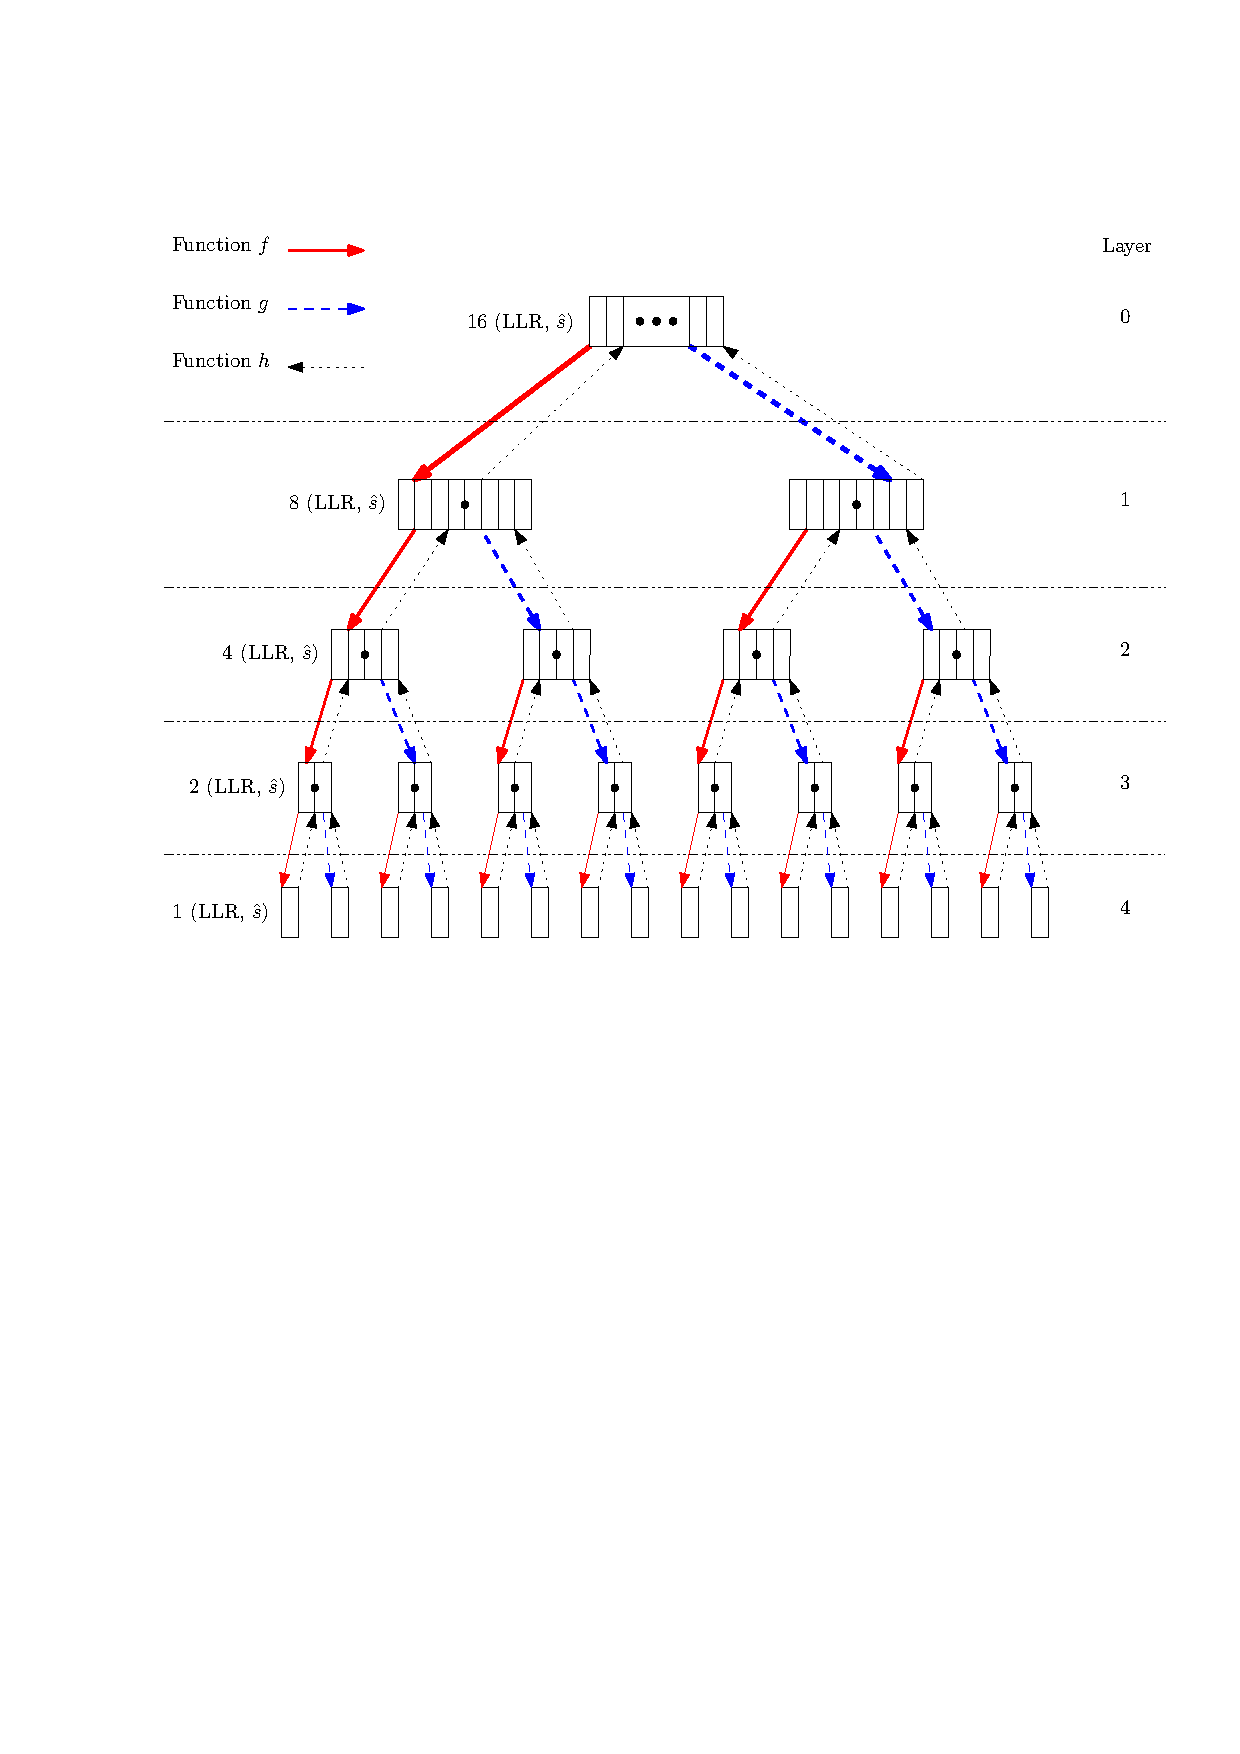
\includegraphics{polar/sc_decoder/sc_decoder}
  \caption{Full SC decoding tree ($N = 16$)}
  \label{fig:alg_polar_sc_decoder}
\end{figure}

The Successive Cancellation (SC) decoding algorithm has been introduced by
\Arikan~\cite{Arikan2009}. It can be seen as the traversal of a binary tree
starting from the root node. For a code length $N=2^m$, the corresponding tree
thus includes $m + 1$ node layers, indexed from $d=0$ (root node layer) down to
$d=m$ (leaf nodes layers). As the tree is initially full, each layer $d$
contains $2^d$ nodes, each node of that layer $d$ containing $2^{m-d}$ LLRs
($\bm{\lambda}$) and $2^{m-d}$ binary values denoted as \textit{partial sums}
($\bm{\hat{s}}$). At the decoder initialization, LLRs received from the channel
($\bm{l}$) are stored in the root node. Then, the decoder performs a pre-order
traversal of the tree. When a node is visited in the downward direction, LLRs of
the node are updated. In the upward direction, partial sums are updated.
Fig.~\ref{fig:alg_polar_sc_decoder} summarizes the computations performed in
both directions. The update functions are:
\begin{eqnarray}
\left\{\begin{array}{l c l c l}
\lambda_c &=& f(\lambda_a,\lambda_b) &=& \lambda_a \boxplus \lambda_b \approx \sign(\lambda_a.\lambda_b).\min(|\lambda_a|,|\lambda_b|)\\
\lambda_c &=& g(\lambda_a,\lambda_b,s)&=&(1-2s)\lambda_a+\lambda_b\\
(\hat{s}_{c}, \hat{s}_{d}) &=& h(\hat{s}_{a}, \hat{s}_{b}) &=& (\hat{s}_{a} \oplus \hat{s}_{b}, \hat{s}_{b}).
\end{array}\right.
\label{eq:alg_polar_f_g_h}
\end{eqnarray}
The $f$ and $g$ functions both generate a single LLR. The $h$ function provides
a couple of partial sums. The $f$ function is the Min-Sum approximation of the
$\boxplus$ operation described in Eq.~\ref{eq:alg_ldpc_ms}. In Polar decoding
using the MS approximation does not significantly impact the decoding
performance. Thus, the MS approximation is privileged.

Before recursively calling itself on the left node, the algorithm applies the
$f$ function; respectively, before calling itself on the right node the $g$
function is applied. At the end (after the recursive call on the right node) the
$h$ function is applied. The $f$ and $g$ functions use the LLRs (read only mode)
from the current node $n_i$ in order to produce the new LLR values into
respectively left and right $n_{i+1}$ nodes. The $h$ function reads the bits
from the left and right $n_{i+1}$ nodes in order to update the bit values of the
$n_i$ node. The $\bm{\lambda}$ LLRs in the leafs are converted in the
$\bm{\hat{s}}$ bits with the hard decision function $\hat{s}_n =
\hardDec(\lambda_n)$.

Leaf nodes are of two kinds: \emph{information bit} nodes and \emph{frozen bit}
nodes. When a frozen bit leaf node is reached, its binary value is
unconditionally set to zero. Instead, when an information leaf node is reached,
its binary value is set according to the \emph{sign} of its LLR (0 if LLR is
positive, 1 otherwise). Once every node in the tree has been visited in both
directions, the decoder eventually updates partial sums in the root node and the
decoding process is terminated. If the polar code is not systematic, the decoded
bits $\bm{\hat{u}}$ are the leaf bits in the tree. Else, if the polar code is
systematic, the decoded bits $\bm{\hat{u}}$ can be directly extracted from the
root node of the polar tree in the form of a $N$-bit partial sum vectors. In the
next sections and chapters, only the systematic polar decoding is considered.

The SC algorithm is a key to construct the polar codes. A density evolution
is performed over the SC binary tree to determine the position of the frozen
bits. The idea is to construct the polar codes according to the decoder
structure. In this manuscript, the Gaussian Approximation (GA) of the density
evolution is used~\cite{Trifonov2012}.

\subsection{Successive Cancellation List Decoding Algorithm}

\begin{algorithm}
  \caption{SCL decoding algorithm.}\label{alg:alg_polar_scl_decoder}

  % \small
  \SetKwProg{Fn}{Function}{}{}

  % \KwIn{$N$ is the frame size.}
  % \KwIn{$L$ is the number of lists (or paths) to maintain.}
  \KwData{$\lambda$ is a 2D buffer ($[L][2N]$) to store the LLRs.}
  \KwData{$\hat{s}$ is a 2D buffer ($[L][N]$) to store the bits.}

  \Fn(\Comment*[f]{$o_{\lambda}$ and $o_{\hat{s}}$ are offsets in $\bm{\lambda}$ and $\bm{\hat{s}}$, resp.}){$\SCLDecode(N, o_{\lambda}, o_{\hat{s}})$}
  {
    $N_{\frac{1}{2}} \gets N / 2$

    \uIf(\Comment*[f]{not a leaf node}){$N > 1$}
    {
      \For(\Comment*[f]{loop over the $L$ paths}){$p=0$ \textbf{to} $L-1$}
      {
        \For(\Comment*[f]{apply the $f$ function}){$i=0$ \textbf{to} $N_{\frac{1}{2}}-1$}
        {
          $\lambda[p][o_\lambda + N + i] \gets f(\lambda[p][o_\lambda + i], \lambda[p][o_\lambda + N_{\frac{1}{2}} + i])$
        }
      }

      $\SCLDecode(N_{\frac{1}{2}}, o_{\lambda} + N, o_{\hat{s}})$ \Comment*[r]{recursive call to the decoder}

      \For{$p=0$ \textbf{to} $L-1$}
      {
        \For(\Comment*[f]{apply the $g$ function}){$i=0$ \textbf{to} $N_{\frac{1}{2}}-1$}
        {
          $\lambda[p][o_\lambda + N + i] \gets g(\lambda[p][o_\lambda + i], \lambda[p][o_\lambda + N_{\frac{1}{2}} + i], \hat{s}[p][o_{\hat{s}} + i])$
        }
      }

      $\SCLDecode(N_{\frac{1}{2}}, o_{\lambda} + N, o_{\hat{s}} + N_{\frac{1}{2}})$ \Comment*[r]{recursive call to the decoder}

      \For{$p=0$ \textbf{to} $L-1$}
      {
        \For(\Comment*[f]{update the partial sums ($h$ function)}){$i=0$ \textbf{to} $N_{\frac{1}{2}}-1$}
        {
          $\hat{s}[p][o_{\hat{s}} + i] \gets h(\hat{s}[p][o_{\hat{s}} + i], \hat{s}[p][o_{\hat{s}} + N_{\frac{1}{2}} + i])$
        }
      }
    }
    \Else(\Comment*[f]{a leaf node})
    {
      $\updatePaths()$ \Comment*[r]{update, create and delete paths}
    }
  }

  $\SCLDecode(N, 0, 0)$ \Comment*[r]{launch the decoder}

  $\selectBestPath()$
\end{algorithm}

The Successive Cancellation List (SCL) algorithm is an evolution of the
SC~\cite{Tal2011}. The SCL algorithm is summarized in
Algorithm~\ref{alg:alg_polar_scl_decoder}. Unlike the SC algorithm, the SCL
decoder builds a list of candidate codewords along the decoding. At each call of
the ``$\updatePaths()$'' sub-routine (l.16), $2L$ candidates are generated. A
path metric is then evaluated to keep only the $L$~best candidates among the
$2L$ paths. The path metrics are calculated as
in~\cite{Balatsoukas-Stimming2015}. At the end of the decoding process, the
candidate codeword with the best path metric is selected in the
``$\selectBestPath()$'' sub-routine (l.18). The decoding complexity of the
SCL algorithm grows as $O(LN\log_2N)$. This linear complexity in L leads to
significant improvements in BER/FER performances compared to the SC decoder,
especially for small code lengths.

\paragraph{CRC Concatenation Scheme}

The authors in~\cite{Tal2011} observed that when a decoding error occurs, the
right codeword is often in the final list, but not with the best path metric.
They proposed to concatenate a CRC to the codeword in order to discriminate the
candidate codewords at the final stage of the SCL decoding. Indeed, this
technique drastically improves the FER performance of the decoder. This
algorithm is denoted as the \emph{CRC-Aided SCL} (CA-SCL). In terms of
computational complexity, the overhead consists in the computation of $L$ CRC at
the end of each decoding.

\subsection{Simplified Successive Cancellation Class of Algorithms}
\label{sec:alg_polar_simplified_decoders}

\begin{figure}[htp]
  \centering
  \includegraphics{polar/tree_pruning_example/tree_pruning_example}
  \caption
    [Example of polar tree pruning on a small binary tree ($N = 8$).]
    {Example of tree pruning on a small binary tree ($N = 8$). The tree is cut
    and the computations are versioned according to the location of the frozen
    bits.}
  \label{fig:alg_polar_tree_pruning_example}
\end{figure}

Frozen bits fully define the decoders leaf values, hence some part of the
traversal can be cut and its computation avoided, depending on the location of
the frozen bits. More generally, the tree functions can be versioned depending
on these bits. In~\cite{Alamdar-Yazdi2011}, a tree pruning technique called the
Simplified SC (SSC) was applied to SC decoding. An improved version was proposed
in~\cite{Sarkis2014a}. This technique relies on the fact that, depending on the
frozen bits location in the leaves of the tree, the definition of dedicated
nodes enables to prune the decoding tree: Rate-0 nodes (\verb|R0|) correspond to
a sub-tree whose all leaves are frozen bits, Rate-1 nodes (\verb|R1|) correspond
to a sub-tree in which all leaves are information bits, REPetition (\verb|REP|)
and Single Parity-Check (\verb|SPC|) nodes correspond to repetition and SPC
codes sub-trees. These special nodes, originally defined for SC decoding, can be
employed in the case of SCL decoding as long as some modifications are made in
the path metric calculation~\cite{Sarkis2016}. This tree-pruned version of the
algorithm is called Simplified SCL (SSCL) and the CA-SSCL when a CRC is used to
discriminate the final candidate codewords. The tree pruning technique can
drastically reduce the amount of computation in the decoding process. The
Fig.~\ref{fig:alg_polar_tree_pruning_example} shows that more than half of the
tree nodes can be removed for $N = 8$ (this is representative of the real-life
codes).

\subsection{Adaptive Successive Cancellation List Decoding Algorithm}

The presence of the CRC can be further used to reduce the decoding time by
gradually increasing $L$. This variation of SCL is called Adaptive SCL
(A-SCL)~\cite{Li2012}. The first step of the A-SCL algorithm is to decode the
received frame with the SC algorithm. Then, the decoded polar codeword is
checked with a CRC. If the CRC is not valid, the SCL algorithm is applied with
$L=2$. If no candidate in the list satisfies the CRC, $L$ is gradually doubled
until it reaches the value $L_{max}$. In this thesis, we call this version of
the A-SCL decoding the Fully Adaptive SCL (FA-SCL) as opposed to the Partially
Adaptive SCL (PA-SCL), in which the $L$ value is not gradually doubled but
directly increased from $1$ (SC) to $L_{max}$. The simplified versions of these
algorithms are denoted PA-SSCL and FA-SSCL. In order to simplify the algorithmic
range, in the remainder of the manuscript, only the simplified versions are
considered. The use of either the FA-SSCL or the PA-SSCL algorithmic improvement
introduces no BER or FER performance degradation as long as the CRC length is
adapted to the polar code length. If the CRC length is too short, the decoding
performance may be degraded because of false detections. These adaptive versions
of SSCL can achieve higher throughputs. Indeed, a large proportion of frames can
be decoded with a single SC decoding. This is especially true when the SNR is
high. This will be further discussed in
Section~\ref{sec:alg_polar_generic_flexible}.

\subsection{Algorithmic Comparison of the Decoders}

\begin{table}[htp]
  \centering
  \caption{Throughput and latency comparison of polar decoding algorithms.}
  \label{tab:alg_polar_algos}
  % {\small
   \begin{tabular}{r c c c}
    \textbf{Decoding}  & \textbf{BER \& FER}   & \multirow{1}{*}{\textbf{Throughput}} & \textbf{Max. Latency}        \\
    \textbf{Algorithm} & \textbf{Performances} & ($\bm{\mathcal{T}}$)                 & ($\bm{\mathcal{L}_{worst}}$) \\
    \hline
    \hline
    SC      & poor      & medium & medium \\
    SSC     & poor      & high   & low    \\
    SCL     & good      & low    & high   \\
    SSCL    & good      & low    & medium \\
    CA-SSCL & very good & low    & medium \\
    PA-SSCL & very good & high   & medium \\
    FA-SSCL & very good & high   & high   \\
  \end{tabular}
  % }
\end{table}

In order to better distinguish all the algorithmic variations, we compare their
main features in Table~\ref{tab:alg_polar_algos}. Each algorithm is
characterized in terms of decoding performance, throughput, and worst case
latency for a software implementation. The non-simplified versions of the
adaptive SCL algorithms are not included in the table for readability.

The SC and especially the SSC algorithms achieve very high throughput and low
latency with poor BER and FER performances. The SCL algorithm improves the
decoding performance compared to the SC algorithm, but its computational
complexity leads to an increased latency and a lower throughput. The SSCL
algorithm improves the decoding throughput and latency without any impact in
terms of BER and FER performances, as long as the tree pruning is not too deep,
as will be discussed in Section~\ref{sec:alg_polar_generic_flexible}. Therefore,
tree pruning is applied to all the following algorithms, namely CA-SSCL, FA-SSCL
and PA-SSCL. By applying CRC to the SCL algorithm, one can achieve better BER
and FER performances at the cost of computational complexity overhead. The
Adaptive SCL algorithms reduce the decoding time with no impact on BER and FER
performances. Furthermore, a tradeoff between throughput and worst case latency
is possible with the use of either PA-SSCL or FA-SSCL decoding algorithms.

\begin{figure}[htp]
  \centering
  \includegraphics[width=0.7\textwidth]{polar/algos_comparison/algos_comparison}
  \caption
    [Decoding performance comparison between CA-SCL and SC decoders.]
    {Decoding performance comparison between CA-SCL and SC decoders.
    Code rate $R = 1/2$, and 32-bit CRC (GZip).}
  \label{plot:alg_polar_algos_comparison}
\end{figure}

CA-SCL decoding performances for large code lengths ($N > 2^{14}$) combined with
large list sizes ($L > 8$) are rarely presented in the literature. This is
probably due to the long simulation time required. The proposed decoders are
integrated in the \AFFECT toolbox. Therefore, multi-threaded and multi-nodes
simulations are enabled to handle such computation-demanding simulations. All
the presented simulations use the Monte Carlo method with a Binary Phase-Shift
Keying (BPSK) modulation. The communication channel is an Additive White
Gaussian Noise (AWGN) channel based on the Mersenne Twister pseudo-random number
generator (MT19937)~\cite{Matsumoto1998} and the Box-Muller
transform~\cite{Box1958}. Figure~\ref{plot:alg_polar_algos_comparison} compares
the BER/FER performances of CA-SCL with SC decoding for a large range of code
lengths. As expected, it appears that the coding gain brought by the SCL
algorithm decreases for larger $N$ values. In the case of $N=2^{16}$, the
improvement caused by the use of the CA-SCL algorithm with $L=32$ and a 32-bit
GZip CRC (\verb|0x04C11DB7| polynomial) instead of SC is about $0.75$ dB
compared to $1.2$ dB with a polar code of size $N=2^{12}$. For larger polar
codes, $N=2^{20}$, the gain is reduced to $0.5$ dB, even with a list depth of
$128$ that is very costly in terms of computational complexity.

The tradeoffs between speed and decoding performance show some general trends.
However, the efficiency of each decoding algorithm is strongly dependent on the
polar code length, code rate, list depth and code construction. It is expected
that the best tradeoff is not always obtained with a single algorithm and
parameter set combination. It is consequently highly relevant to use a generic
and flexible decoder, that supports all variants of the decoding algorithms.
Thus, it is possible to switch from one to another as shown in the following
section.

\subsection{Generic and Flexible Decoders}
\label{sec:alg_polar_generic_flexible}

One of the main contribution of this thesis lies in the flexibility and the
genericity of the proposed software decoder. These terms need to be clearly
defined in order to circumvent possible ambiguity. In the remainder of the
manuscript, the \textit{genericity} of the decoder concerns all the parameters
that define the supported polar code such as the codeword length, the code rate,
the frozen bits set, the puncturing patterns and the concatenated CRC. These
parameters are imposed by the telecommunication standard or the communication
context. In the wireless communications context, these are constantly adapted by
AMC methods~\cite{Dahlman2013}. In this work, a decoder is considered
\textit{generic} if it is able to support any combination of these parameters
that can be changed during a real time execution. On the other hand, the
\textit{flexibility} of a decoder includes all the customizations that can be
applied to the decoding algorithm for a given polar code: variant of the
decoding algorithm, data quantization, list size $L$, tree pruning strategy, ...
These customizations are not enforced by a standard. The flexibility gives some
degrees of freedom to the decoder in order to find the best tradeoff between
decoding performance, throughput or latency for a given polar code.

\subsubsection{Genericity}

In the context of wireless communications, the standards define several
different code lengths~$N$ that have to be supported to share bandwidth between
different users. This is also the case for the code rate $R$ that needs to be
adapted to the quality of the transmission channel. Therefore, a practical
implementation should be adapted to both $N$ and $R$ in real-time in order to
limit latency.

A polar code is completely defined by $N$ and the frozen bits set
$\bm{u}_{\mathcal{A}^c}$. Several methods exist to generate some "good" sets of
frozen bits~\cite{Tal2013,Trifonov2012}. The code rate $R$ depends on the size
of $\bm{u}_{\mathcal{A}^c}$. In their original form, polar code lengths are only
powers of two. The puncturing and shortening techniques
in~\cite{Wang2014,Niu2013,Miloslavskaya2015} enable to construct polar codes of
any length at the cost of slightly degraded decoding performance. The coding
scheme can be completed with the specification of a CRC.

The proposed decoders are generic regarding the code dimension $K$, the code
length $N$, the frozen bits set $\bm{u}_{\mathcal{A}^c}$ and the puncturing
patterns. All of them are dynamic parameters of the decoders and can be defined
in input files. All CRC listed in~\cite{CRCWiki2017} are available along with
the possibility to define others. It is shown in~\cite{Zhang2017} that custom
CRCs for polar codes can have a very good impact on the decoding performance.

Relying on an unique software description also implies that the tree pruning
technique has to be dynamically defined. Indeed, this technique depends on the
frozen bits set $\bm{u}_{\mathcal{A}^c}$. Not sacrificing throughput or latency
while maintaining the genericity is at the core of the proposed implementation.
Flexibility in terms of decoding algorithms, described in the following, is
necessary to deal with this challenge.

\subsubsection{Flexibility}

On the one hand, the reason for the decoder genericity is the compliance to the
telecommunication standards. On the other hand, the flexibility of the decoder
regroups several algorithmic variations that are discussed in the following.
These variations allow several tradeoffs of multiple sorts, whatever the
standard. They are all included in a single source code.

In the proposed decoders the following parameters can be changed dynamically
without re-compilation: the list size $L$, the tree pruning strategy, the
quantization of the LLRs and the different SCL variants. Each of these
adjustments can be applied to access to different tradeoffs between throughput,
latency, and error rate performance. As a consequence, one can easily fine-tune
the configuration of the software decoder for any given polar code.

\paragraph{List Size}

\begin{figure}[htp]
  \centering
  \includegraphics[width=0.70\textwidth]{polar/scl_l/scl_l}
  \caption
    [Tradeoffs between CA-SSCL decoding and throughput performances.]
    {Tradeoffs between CA-SSCL decoding and throughput performances depending on
    $L$. $N=2048$, $R=0.5$, and 32-bit CRC (GZip). For $L=1$, the SSC decoder is
    used with a ($2048$,$1024$) polar code.}
  \label{plot:alg_polar_scl_l}
\end{figure}

As mentioned earlier, the list size $L$ impacts both speed and decoding
performance. In Figure~\ref{plot:alg_polar_scl_l}, the throughput as well as BER
and FER performances of the CA-SSCL algorithm are shown for different $L$
values. A ($2048$,$1024$) polar code with a 32-bit CRC is considered. The
computational complexity increases linearly with $L$: the throughput is
approximately halved when $L$ is doubled, except for the case of the SC
algorithm ($L=1$) which is much faster. Indeed, there is no overhead due to the
management of different candidate paths during the decoding. For $L\geq4$ and
$E_b/N_0=2$, the FER is also approximately halved when the list size $L$ is
doubled.

\paragraph{Tree Pruning Strategy}

A second degree of flexibility is the customization of the SCL tree pruning. The
authors in~\cite{Alamdar-Yazdi2011,Sarkis2016} defined dedicated nodes to prune
the decoding tree and therefore to reduce the computational complexity. In this
proposed decoder, each dedicated node can be activated separately. The ability
to activate dedicated nodes at will is useful in order to explore the
contribution of each node type on the throughput.

\paragraph{LLR Quantization}

\begin{figure}[htp]
  \centering
  \includegraphics[width=0.70\textwidth]{polar/scl_bfer/scl_bfer_rep}
  \caption
    [Impact of the \texttt{REP} node size on fixed-point SSCL decoding.]
    {Impact of the \texttt{REP} node size on fixed-point SSCL decoding.
    Code ($2048$,$1723$), $L=32$.}
  \label{plot:alg_polar_scl_bfer_rep}
\end{figure}

Another important parameter in both software and hardware implementations is the
quantization of data in the decoder. The quantization of LLRs and partial sums
in the decoder have an impact on decoding performance. Quantized implementations
of the SC algorithm have been proposed in~\cite{Giard2016} but to the best of
our knowledge, the proposed decoder is the first SCL software implementation
that can benefit from the 8-bit and 16-bit fixed-point representations of LLRs
and internal path metrics. In the 8-bit mode LLRs and path metrics are saturated
between $-127$ and $+127$ after each operation. Moreover, to avoid overflows,
the path metrics are normalized after each ``$\updatePaths()$'' call (cf.
Alg.~\ref{alg:alg_polar_scl_decoder}) by subtracting the smallest metric to each
one of them. Figure~\ref{plot:alg_polar_scl_bfer_rep} shows the BER and FER
performances of the CA-SSCL decoder for 32-bit floating-point, 16-bit and 8-bit
fixed-point representations. One can observe that the \verb|REP| nodes degrade
the decoding performance in a 8-bit representation because of accumulation (red
triangles curve). Indeed, it is necessary to add all the LLRs of a \verb|REP|
node together in order to process it, which may lead to an overflow in the case
of fixed-point representation. It can happen when the size of the repetition
nodes is not limited ($\texttt{REP}_\texttt{2+}$). However, the size limitation
of the repetition nodes to 8 ($\texttt{REP}_\texttt{8-}$) fixes this issue.

\paragraph{Supporting Different Variants of the Decoding Algorithms}

Besides the $L$ values, the tree pruning and quantization aspects, the proposed
software polar decoder supports different variants of the SCL algorithm:
CA-SSCL, PA-SSCL, FA-SSCL.

\begin{figure}[htp]
  \centering
  \includegraphics[width=0.70\textwidth]{polar/scl_adaptive/scl_adaptive}
  \caption
    [FER and throughput of the Fully and Partially Adaptive SSCL decoders.]
    {Frame Error Rate (FER) performance and throughput of the Fully and
    Partially Adaptive SSCL decoders (FA and PA). Code ($2048$,$1723$) and
    32-bit CRC (GZip). 32-bit floating-point representation.}
  \label{plot:alg_polar_scl_adaptive}
\end{figure}

As shown in~\cite{Sarkis2016}, the adaptive version of the SCL algorithm yields
significant speedups, specially for high SNR. The original adaptive SCL
described in~\cite{Li2012}, denoted as Fully Adaptive SCL (FA-SSCL) in this
work, gradually doubles the list depth $L$ of the SCL decoder when the CRC is
not valid for any of the generated codewords at a given stage until the value
$L_{max}$. By contrast, the adaptive decoding algorithm implemented
in~\cite{Sarkis2016}, called in this manuscript Partially Adaptive SCL
(PA-SSCL), directly increases the list depth from $1$ (SC) to $L_{max}$. In
Figure~\ref{plot:alg_polar_scl_adaptive}, the two versions (FA-SSCL and PA-SSCL)
are compared on a ($2048$,$1723$) polar code and 32-bit CRC (GZip). The LLRs
values are based on a 32-bit floating point representation. Note that as the FER
performance of PA-SSCL and FA-SSCL are exactly the same, the related error
performance plots completely overlap. The throughput of the FA-SSCL algorithm is
higher than that of the PA-SSCL algorithm for some SNR values, depending on the
code parameters. Considering typical FER values for wireless communication
standards ($10^{-3}$ to $10^{-5}$), in the case of a ($2048$,$1723$) polar code,
the throughput of FA-SSCL is double that of PA-SSCL with $L = 8$, while it is
multiplied by a factor of $7$ with $L=32$. The drawback of FA-SSCL is that
although the average latency decreases, the worst case latency increases.

\begin{figure}[htp]
  \centering
  \includegraphics[width=0.70\textwidth]{polar/scl_bfer/scl_bfer_crc}
  \caption{Impact of the CRC size on SCL and A-SCL decoding. Code ($2048$,
    $1723$), $L=32$.}
  \label{plot:alg_polar_scl_bfer_crc}
\end{figure}

The adaptive versions of the algorithm achieve better throughputs, but CA-SCL
may also be chosen depending on the CRC. One may observe in
Figure~\ref{plot:alg_polar_scl_bfer_crc} that an adaptive decoder dedicated to
an 8-bit CRC with a ($2048$,$1723$) polar code and $L=32$ leads to a loss of
$0.5$ dB for a FER of $10^{-5}$ compared to its non adaptive counterpart.

Both polar code genericity and decoding algorithm flexibility are helpful to
support the recommendations of wireless communications in an SDR or Cloud-RAN
context. The code and decoder parameters can be dynamically changed in the
proposed decoder, while maintaining competitive throughput and latency.
However, depending on the constraints of the communication system, if the main
objective is to reach high throughputs and low latency decoding, it is possible
to trade some of the genericity and the flexibility for increased performance.
The next section discusses the polar decoder unrolling strategy.

\subsection{Unrolled Decoders}

The tree structure at the heart of SC and SCL decoders is fully determined by
the parameters of a given code instance: the code size, the code rate ($R = K /
N$), position of the frozen bits. All these parameters are statically known at
compile time. The recursive tree traversal code structure and the corresponding
tree data structure are challenging to optimize for a compiler. It is then
possible to completely flatten all the recursive calls in the tree. This leads
to a specific generated polar decoder where the $N$, $K$, $R$, the frozen bits
set, the puncturing pattern, and the CRC are fixed. This technique has been used
in previous works for both SC and SCL decoders~\cite{Sarkis2014,Cassagne2015c,
Cassagne2016b,Sarkis2016} and demonstrated higher efficiency than the generic
and flexible approach in terms of decoding throughputs and latencies. Depending
on the number of different configurations to support in a communication
standard, it is still possible to generate one specific unrolled decoder per
configuration.

\section{Turbo Codes}
\label{sec:alg_turbo}

\subsection{Coding Scheme}

In this sub-section, the convolutional sub-encoder is presented first and then
the turbo encoding process is detailed. The first convolutional codes have been
introduced by Peter Elias in 1955~\cite{Elias1955}. The objective was to propose
an alternative to block codes in term of codeword length flexibility:
theoretically, the length of a convolutional code is infinite. The coding scheme
output depends on the current input and on the inputs before.

\begin{figure}[htp]
  \centering
  \subfloat[][Encoding graph.]
  {
    \includegraphics[scale=1.0]{turbo/sub_encoder/sub_encoder}
    \label{fig:alg_turbo_sub_encoder_graph}
  }
  \quad
  \subfloat[][Mealy's machine.]
  {
    \includegraphics[scale=0.75]{turbo/mealy/mealy}
    \label{fig:alg_turbo_sub_encoder_mealy}
  }
  \\
  \subfloat[][Trellis representation.]
  {
    \includegraphics[scale=0.9]{turbo/trellis/trellis}
    \label{fig:alg_turbo_sub_encoder_trellis}
  }
  \caption{Example of a recursive and systematic convolutional encoder ($R =
    1/2$).}
  \label{fig:alg_turbo_sub_encoder}
\end{figure}

For a $R=1/2$ encoder, the current $p_k$ output parity bit can be expressed as a
linear combination of the $\nu$ previous bits of the message:
$p_k = \sum_{j=0}^\nu g^{(2)}_{j} u_{k-j} + \sum_{j=1}^\nu g^{(1)}_{j} p_{k-j}$,
where $\nu$ represents the number of elements memorized inside the encoder.
The sequence of elements $g_j$ is called the code-generating sequence and is
often given in octal. Fig.~\ref{fig:alg_turbo_sub_encoder_graph} presents a
convolutional encoder of rate $R = 1/2$ with a memory $\nu = 2$ ($D_0$ and $D_1$
are shift registers). Its two code-generating sequences $\bm{g^{(1)}} = (7)_8$
and $\bm{g^{(2)}} = (5)_8$ define the $c_2 = p$ output while $c_1 = u$. In
the example, the encoder has the particularity to be systematic because
$c_1 = u$ and recursive because of the feedback loop before the first shift
register $D_0$. In the literature, this type of coding scheme is called
Recursive Systematic Convolutional (RSC). Only RSC codes are considered in the
document. In Fig.~\ref{fig:alg_turbo_sub_encoder}, the number of $D$ memories
$\nu = 2$ and so, the encoder has $2^\nu = 4$ different states. Thus, a
convolutional encoder can be seen as a Mealy's machine (or a finite-state
machine) as shown in Fig.~\ref{fig:alg_turbo_sub_encoder_mealy}. The initial
state $S_0$ corresponds to $D_0 = 0$ and $D_1 = 0$, the state~$S_1$ corresponds
to $D_0 = 1$ and $D_1 = 0$, the state~$S_2$ corresponds to $D_0 = 0$ and
$D_1 = 1$ and, finally, the state~$S_3$ corresponds to $D_0 = 1$ and $D_1 = 1$.
The notation on the edges is in the form of $u/c_1c_2$. For instance, from the
state~$S_1$, if the input bit $u$ is 1, then the encoder will output two bits
$c_1 = 1$ and $c_2 = 0$ and will go in the state~$S_2$: this is denoted by
\emph{1/10} below the directed edge between $S_1$ and $S_2$.

Fig.~\ref{fig:alg_turbo_sub_encoder_trellis} introduces a new representation of
convolutional encoders: the trellis. This representation has been used the first
time by Dave Forney in 1973~\cite{Forney1973}. It is especially useful to
facilitate the understanding of the decoding process as it allows to see the
internal state of the encoder, its transitions, and the temporal evolution.
However, the purpose of this chapter is not to detail the decoding process, it
will be made in the next chapter. Considering the encoder initial state $S_0$,
from $t = 0$ the two next possible states are $S_0$ and $S_1$. At $t = 1$, the
encoder can be in state $S_0$ or $S_1$, so the next possible states are $S_0$,
$S_1$, $S_2$ or $S_3$. One can note that starting from $\nu +1$ time units, the
trellis pattern is repeated.

\begin{figure}[htp]
  \centering
  \includegraphics{turbo/encoder/encoder}
  \caption{Turbo encoder ($R = 1/3$) with two convolutional sub-encoders and a
    $\Pi$ interleaver.}
  \label{fig:alg_turbo_encoder}
\end{figure}

As mentioned before, a turbo encoder is built from two convolutional
sub-encoders. The sub-encoders can be different but it is rare.
Fig.~\ref{fig:alg_turbo_encoder} shows a generic view of the turbo encoding
process. In the example, the code rate of the turbo encoder is $R = 1/3$. This
rate is obtained from two convolutional sub-encoders of rate $R = 1/2$ (like the
one shown in Fig.~\ref{fig:alg_turbo_sub_encoder}). The two parity bits $p$ and
$p'$ are obtained from the $c_2$ outputs of the convolutional sub-encoders while
the systematic $c_1$ outputs are ignored. The first sub-encoder encodes the
$u$ input bit while the second one encode the $u'$ bit. The $u'$~bit is
determined from $u$ after the $\Pi$ interleaving process. For each $u_k$ bit
there is a single $u_k'$ associated bit in the $K$ input information bits. The
interleaving process is a key point of the decoding performance in the turbo
coding scheme, its main purpose is to fight against chunks of errors. During the
interleaving process the sequence of information bits is in the \emph{natural
order}, then these bits are permuted and the interleaver outputs a sequence of
information bits in the \emph{interleaved order}. The permutation function
defines the interleaver type. The $K$ information bits in the natural order are
given to the sub-encoder 1 while the $K$ information bits in the interleaved
order are given to the sub-encoder 2.

\subsection{Turbo Decoding Algorithm}
\label{sec:turbo_overview}

\begin{figure}[htp]
  \centering
  \includegraphics[scale=1.0]{turbo/decoder/decoder}
  \caption{Structure of a turbo decoder.}
  \label{fig:alg_turbo_decoder}
\end{figure}

The turbo decoder consists of two concatenated component decoders exchanging
soft information in terms of log-likelihood ratio (LLR) for each transmitted
information bit through an interleaver and a deinterleaver.
Fig.~\ref{fig:alg_turbo_decoder} illustrates the internal structure of a turbo
decoder. Two Soft Input Soft Output (SISO) decoders are represented with the
interleaving process $\Pi$ and the deinterleaving process $\Pi^{-1}$. In this
manuscript, we will only consider rate $R = 1/3$ codewords. $K$ represents the
number of information bits and $N$ is the codeword size: $N = K \times 3$.

\paragraph{Algorithm Outline}

Turbo decoding is carried out in multiple iterations where each iteration
consists of two component decoding phases. In each phase, a component
decoder performs a maximum a posteriori (MAP) decoding using the BCJR algorithm
\cite{Bahl1974}, which generates so-called extrinsic LLRs given the LLRs
obtained by the detector and a priori LLRs obtained from the other component
decoder. The BCJR algorithm consists of one forward and one backward traversal
on a trellis, which is defined by the underlying code. Specifically, to decode a
codeword of $K$ information bits, the BCJR algorithm performs the following
steps: (i) the branches of the trellis are weighted from the systematic LLRs
($\bm{L_s}$), the parity LLRs ($\bm{L_p}$) and the a priori information
($\bm{L_a}$); (ii) in the forward traversal step, it iteratively computes $K$
sets of forward state metrics for each transmitted information bit; (iii) in the
backward traversal step, it iteratively computes $K$ sets of backward state
metrics for each transmitted information bit; (iv) to compute the extrinsic LLRs
($L_e$), the BCJR algorithm then combines the forward and backward state
metrics. The $\bm{L_s}$, $\bm{L_p}$, $\bm{L'_p}$ vectors of LLRs correspond to
the decoder input $\bm{l}$ split in 3 sub-sets.

\begin{algorithm}
  \caption{Pseudo-code of the BCJR decoding algorithm.}
  \label{alg:alg_turbo_bcjr}

  % \small
  % \For(\Comment*[f]{Sequential loop}){$\text{all~frames}$}
  % {
    \For(\Comment*[f]{(i) parallel loop}){$k=0;~k<K;~k=k+1$}
    {
      $\boldsymbol{\gamma}^k\gets \computeGamma(L_{s}^k, L_{p}^k, L_{a}^k)$
    }

    $\boldsymbol{\alpha}^0\gets \initAlpha()$

    \For(\Comment*[f]{(ii) sequential loop}){$k=1;~k<K;~k=k+1$}
    {
      $\boldsymbol{\alpha}^k\gets \computeAlpha(\boldsymbol{\alpha}^{k-1}, \boldsymbol{\gamma}^{k-1})$
    }

    $\boldsymbol{\beta}^{K-1}\gets \initBeta()$

    \For(\Comment*[f]{(iii) sequential loop}){$k=K-2;~k \geq 0;~k=k-1$}
    {
      $\boldsymbol{\beta}^k\gets \computeBeta(\boldsymbol{\beta}^{k+1}, \boldsymbol{\gamma}^{k})$
    }

    \For(\Comment*[f]{(iv) parallel loop}){$k=0;~k<K;~k=k+1$}
    {
      $L_e^k\gets \computeExtrinsic(\boldsymbol{\alpha}^k, \boldsymbol{\beta}^{k}, \boldsymbol{\gamma}^{k}, L_{s}^k, L_{a}^k)$
    }
  % }
\end{algorithm}

Algorithm~\ref{alg:alg_turbo_bcjr} resumes the previously enumerated steps in
a pseudo-code. $\bm{\gamma}$ are the values of the trellis branches,
$\bm{\alpha}$ are the values of the nodes in the forward traversal of the
trellis and $\bm{\beta}$ are the values of the nodes in the backward traversal
of the trellis.

\begin{figure}[htp]
  \centering
  \includegraphics[width=1.0\textwidth]{turbo/encoder_lte/encoder_lte}
  \caption
    [Turbo LTE encoder and its associated 8-state trellis.]
    {Turbo LTE encoder and its associated 8-state trellis.
     $\bm{g^{(1)}} = (13)_8$, $\bm{g^{(2)}} = (15)_8$.}
  \label{fig:alg_turbo_encoder_lte}
\end{figure}

In this thesis, we focus on the turbo codes of the LTE standard~\cite{ETSI2013}
(3G and 4G mobile networks). Fig.~\ref{fig:alg_turbo_encoder_lte} gives the
definition of the LTE turbo encoder. This encoder leads to a 8-state trellis. In
the next sections and chapters, the LTE trellis is always considered.

\paragraph{Branch-metric Computations}

Let $S_j^{k+1}$ be the $j^{th}$ state associated with information bit $k+1$ and
$j \in \{0,7\}$. There are two incoming branches into state $S_j^{k+1}$. Each
incoming branch is associated with values $u^k$ and $p^k$, the $k^{th}$
information bit and the parity bit (both $\pm1$), respectively. The branch
metrics associated with states $S_i^k$ and $S_j^{k+1}$ are computed as follows:
\begin{equation}
\label{eq:alg_turbo_gamma}
 \gamma(S_i^k, S_j^{k+1}) = 0.5(L_{s}^k + L_a^k)u^k + 0.5(L_p^k p^k).
\end{equation}
Here, $L_{s}^k$ and $L_a^k$ are the systematic channel LLR and the a priori
LLR for $k^{th}$ trellis step, respectively.
In the BCJR SISO decoder 1, the $\bm{L_{s}}$, $\bm{L_{p}}$ and $\bm{L_{a}}$
vectors of LLRs are considered (natural domain) while in the BCJR SISO decoder
2, the $\bm{L'_{s}}$, $\bm{L'_{p}}$ and $\bm{L'_{a}}$ LLRs are used instead
(interleaved domain). However, the computations in the natural and in the
interleaved domain are similar, this is why only the operations in the natural
domain are given here. Note that we do not need to evaluate the branch metric
$\gamma(s^k , s^{k+1})$ for all 16 possible branches, as there are only four
different branch metrics:
$\gamma^k_0 = 0.5(L_{s}^k + L_a^k + L_p^k)$,
$\gamma^k_1 = 0.5(L_{s}^k + L_a^k - L_p^k)$, $-\gamma^k_0$, and $-\gamma^k_1$.

\paragraph{Forward and Backward State-metric Computations}

The forward state metrics can be computed iteratively from trellis step to
trellis step. The forward state metrics of step $k+1$ correspond to the vector
$\bm{\alpha^{k+1}} = [\alpha_0^{k+1}, ... ,\alpha_7^{k+1}]$, where the
$j^{th}$ forward state metric $\alpha_j^{k+1}$ only depends on two forward
state metrics of stage $k$. These state metrics are computed by:
\begin{equation}
  \label{eq:alg_turbo_alpha}
  \alpha_j^{k+1} =
  \maxstar_{i \epsilon F} ( \alpha_i^k + \gamma(S_i^k, S_j^{k+1}) ),
\end{equation}
where the set $F$ contains the two indexes of the states in step $k$ connected
to state $S_j^{k+1}$ (as defined by the trellis). The $\maxstar$ operator is
defined as:
\begin{equation}
   \maxstar(a,b) = \max(a,b) + \log(1 + \exp(-|a-b|)),
\end{equation}
where $\log(1 + \exp(-|a-b|))$ is a correction term.
Computation of the backward state metrics is similar to that of the forward
trellis traversal in Eq.~\ref{eq:alg_turbo_alpha}. The vector of backward state
metrics, denoted by $\bm{\beta^k} = [\beta_0^k, ..., \beta_7^k]$, is
computed as:
\begin{equation}
  \label{eq:alg_turbo_beta}
  \beta_j^k =
  \maxstar_{i \epsilon B} ( \beta_i^{k+1} + \gamma(S_j^k, S_i^{k+1}) ),
\end{equation}
where $B$ is the set containing the indexes of states in step $k+1$ connected to
state $S_j^k$ as defined by the trellis.

\paragraph{Extrinsic LLR Computations}

After the forward and backward iterations have been carried out, the extrinsic
LLRs for the $k^\text{th}$ bit are computed as:
\begin{equation}
  \label{eq:alg_turbo_ext}
  \begin{aligned}
  L_e^k = \maxstar_{\{S_k, S_{k+1}\}\epsilon U^1}\big( \alpha_i^k + \beta_j^{k+1} +
  \gamma(S_i^k, S_j^{k+1}) \big) \\
  - \maxstar_{\{S_k, S_{k+1}\}\epsilon U^{-1}}\big( \alpha_i^k + \beta_j^{k+1} +
  \gamma(S_i^k, S_j^{k+1}) \big) \\
  - L_{s}^k - L_a^k,
  \end{aligned}
\end{equation}
where the sets $U^1$ and $U^{-1}$ designate the set of states connected by paths
where $u^k=1$ and the set of states connected by paths where $u^k=-1$,
respectively (because of the BPSK modulation).

\begin{figure}[htp]
  \centering
  \includegraphics[width=0.7\textwidth]{turbo/iterations/iterations}
  \caption
    [Decoding performance of the turbo decoder depending on the number of
     iterations.]
    {Decoding performance of the turbo decoder depending on the number of
     iterations. LTE code, $K = 6144$, $R = 1/3$, MAP algorithm.}
  \label{plot:alg_turbo_iterations}
\end{figure}

Fig.~\ref{plot:alg_turbo_iterations} shows the decoding performance of the turbo
decoder depending on the number of iterations. The biggest code from the
LTE standard is evaluated ($K = 6144$ and $R=1/3$). It has been shown that the
BCJR is in fact an instance of the BP algorithm~\cite{McEliece1998}. In one
iteration, the BCJR decoder 1 and 2 are run. Thus, the computational complexity
of one turbo decoding iteration is higher than one LDPC BP decoding iteration.

\paragraph{Approximation of the MAP Operations in the BCJR Decoder}

\begin{figure}[htp]
  \centering
  \includegraphics[width=0.7\textwidth]{turbo/approximations/approximations}
  \caption
    [Decoding performance of the turbo decoder depending on the approximations.]
    {Decoding performance of the turbo decoder depending on the BCJR algorithm
     approximations. The maximum a posteriori (MAP), the max-log-MAP (ML-MAP)
     and the enhanced max-log-MAP (EML-MAP, $\alpha = 0.75$) are evaluated.
     $K = 6144$, $R=1/3$ and 6 decoding iterations.}
  \label{plot:alg_turbo_approximations}
\end{figure}

The $\maxstar$ operator of the MAP algorithm is compute intensive, mainly due to
the logarithm and exponential functions in the correction term. It can be
approximated as follow: $\maxstar(a,b) \approx \max(a,b)$. The correction term
is simply removed. This approximation is called the \emph{max-log-MAP} algorithm
(ML-MAP). Its low computational complexity makes efficient software and hardware
implementations possible. However, the ML-MAP algorithm negatively affects the
decoding performance. It this then possible to partially recover the error-rate
performance loss by scaling the extrinsic LLRs in the turbo decoder by a factor
$\alpha$: this is called the \emph{Enhanced} max-log-MAP (EML-MAP)
algorithm~\cite{Vogt2000,Studer2011}. The impact of the approximations on the
decoding performance is shown in Fig.~\ref{plot:alg_turbo_approximations}.

\paragraph{Impact of the Quantification on the Error-rate}

\begin{figure}[htp]
  \centering
  \includegraphics[width=0.7\textwidth]{turbo/quantification/quantification}
  \caption
    [BER and FER of the turbo decoder for $K = 6144$ (6 iters) and $R=1/3$.]
    {Bit Error Rate (BER) and Frame Error Rate (FER) of the decoder for $K =
    6144$, $R=1/3$ and 6 decoding iterations. Enhanced max-log-MAP algorithm
    ($\alpha = 0.75$).}
  \label{plot:alg_turbo_quantification}
\end{figure}

Fig.~\ref{plot:alg_turbo_quantification} shows the decoding performance of the
turbo decoder depending on the quantification. \emph{float} is the ideal
decoding performance of the EML-MAP algorithm on 32-bit floating-point.
\emph{int-16} is a quantified version of the decoder, on 16-bit and with
fixed-point arithmetic computations. Before to enter in the decoder, the
$\bm{l}$~LLRs are converted from a floating-point representation to a
fixed-point representation: they are saturated on $s = 6$ bits, of which $v = 3$
bits are dedicated to the fractional part ($Q_{s,v}$). Inside the decoder, the
saturation is made over 16 bits ($s = 16$). One can note that there is no
decoding performance degradation. Finally, \emph{int-8} is the 8-bit quantified
version of the decoder. Compared to the 16-bit version, the fractional part of
the 8-bit version is represented with 2 bits ($Q_{6,2}$) instead of 3. The
internal saturations are on 8-bit. This version shows a 0.1 dB degradation. The
limited dynamic of 8-bit format together with early saturation inside the
decoder are responsible for this small performance loss.

\section{Sparse Code Multiple Access}
\label{sec:alg_scma}

\subsection{Presentation and Related Works}

Non-Orthogonal Multiple Access (NOMA) mechanisms are investigated as means to
improve the fifth-generation mobile communication systems (5G)~\cite{Islam2017}
to realize massive connectivity and to reduce bit error rates. Sparse Code
Multiple Access (SCMA) is a NOMA mechanism that offers better bit error rate
performance and higher spectral efficiency, while the sparsity of the codebooks
ensures lower complexity of decoding compared to other non-orthogonal
modulations~\cite{Nikopour2013}. SCMA is a promising candidate for 5G
communication systems since it provides up to 3 times more connectivity by
spreading the information of each user's codebook over sets of shared OFDM
frequency tones~\cite{Altera2015}. According to the NGMN white
paper~\cite{Alliance2015}, 5G targets more diverse scenarios compared to 4G.
Applications can be broadband support in dense areas, low latency connectivity
for Augmented Reality (AR) and reliable communication for intelligent industrial
controls, Internet of Things (IoT) or Internet of Mission Critical Things
(IoMCT). Unfortunately, the massive connectivity and spectral efficiency of SCMA
come at the cost of high complexity in the decoder, making the design of high
throughput and low complexity decoders a challenge~\cite{Lu2015}.

Exploiting sparsity of the codebooks, Belief Propagation (BP) or Message Passing
Algorithm (MPA) decoders were introduced to achieve near Maximum Likelihood
performance with lower complexity~\cite{Zhang2014a}. Substantial research works
were conducted on improving SCMA decoders to satisfy the uplink requirements of
5G. Indeed, MPA is populated with many exponential computations to compute the
extrinsic information and probabilities of the received signal. This is based on
modeling the channel noise with a Gaussian probability density function (PDF). A
classical improvement to this bottleneck is the computation of extrinsic
information in the logarithm domain, which led to develop the log-MPA decoder.
In~\cite{Liu2016}, fixed-point and floating-point implementations of the MPA and
log-MPA on FPGA are studied. The bit error rate performance and complexity of
the MPA and log-MPA are compared and it is concluded that using log-MPA with 4
message passing iterations achieves a good tradeoff between performance and
complexity. In~\cite{Bayesteh2015}, several complexity reduction techniques are
proposed to increase the system throughput. These techniques are 1) SCMA
codebook design with minimum number of projections, 2) clustered MPA (CMPA)
which defines sub-graphs in MPA and runs MPA on them, and 3) selected
exponential computations. In~\cite{Du2016} an adaptive Gaussian approximation
is used to unselect the edges of the graph with smaller modulus. In addition,
mean and variance feedbacks are employed to compensate information loss caused
by unselected edges. User's codebooks play an important role for fast
convergence of the MPA or log-MPA. As investigated in~\cite{Taherzadeh2014,
Peng2017,Yan2017}, revisiting codebook design can help to reduce the number of
iterations needed for MPA decoding of SCMA. In~\cite{Jia2018}, an improved MPA
is proposed which eliminates determined user codewords after a certain number of
iterations and continue the iterations for undetermined user's codewords.
Similarly, in~\cite{Yang2016}, a belief threshold is set to choose the most
reliable edge probabilities and continue the iterations for the others. A
Shuffled MPA (S-MPA) is introduced in~\cite{Du2016a}. S-MPA is based on
shuffling the messages between function nodes and variable nodes. As a result,
the convergence rate is accelerated. A Monte Carlo Markov Chain Method is
proposed in~\cite{Chen2016} to decode SCMA signals and sphere decoding is also
explored in~\cite{Yang2017,Wei2017} for SCMA receiver design.

The main difference between this work and previously cited works is to combine
an analytic view of MPA complexity with hardware and resource aware programming,
and to exploit hardware features available in general purpose processors (GPPs).
The SCMA decoding algorithms are revised in light of the needs of Cloud Radio
Access Networks (Cloud-RANs).

% The main difference between this work and previously cited works is that the
% present manuscript combines an analytic view of MPA complexity with hardware and
% resource aware programming, exploiting hardware features available in general
% purpose processors (GPPs). The SCMA decoding algorithms are revised in light of
% the needs of Cloud Radio Access Networks (Cloud-RANs) and to take full advantage
% of key hardware features available in GPPs such as their SIMD engine. In the
% early 2000s, the performance of many processors improved significantly due to
% clock rate increases. This increase of performance needed very minimal if any
% programming effort, however the drawbacks of high clock rate was more power and
% energy consumption, overheating of processors, leakage currents and signal
% integrity problems. These disadvantages led designers to follow new paradigms
% such as thread-level and data-level parallelisms that provide good performance
% at lower clock speeds. Another challenge was data access efficiency in cache and
% RAM for performance critical algorithms. Higher performance also came from
% improved cache access efficiency of heterogeneous processors and parallel access
% to the L1 cache through vectorized instructions. Therefore, complicated and
% control heavy algorithms such as MPA have to be adapted for efficient execution
% on heterogeneous architectures and their exploitable parallelism must be
% expressed at every level of the code, whether in arithmetic or memory access
% instructions. Particularly, various Single Instruction Multiple Data (SIMD)
% extensions and thread-level parallelism are used to increase the throughput of
% MPA decoding on various platforms.

% This work reports on two contributions that can be useful for any variation of
% the aforementioned MPA. First, MPA and log-MPA have been adapted to use SIMD
% extensions leveraging the available data-level parallelism. The algorithms are
% revised to have aligned and contiguous access to memory, which is crucial to
% achieve high memory throughput. Various SIMD instruction set architectures
% (ISAs) such as Advanced Vector Extensions (AVX), Streaming SIMD Extension (SSE),
% Knights Corner Instruction (KNCI) and ARM\R NEON are used to enhance the
% performance of various parts of the algorithm. Multi-threaded programming
% technique and power efficiency are also studied in this paper.

% Second, efforts have been made to reduce the high dynamic ranges and high
% storage burden that are induced by the numerous calculations of the exponential
% function embedded in MPA, which is one of its main points of congestion. To
% eliminate calculations of the exponentials in the MPA, this paper uses
% approximate modeling of noise. Indeed, a Gaussian Probability Density Function
% (PDF) is estimated with sub-optimal, bell shaped, polynomial PDFs. Using
% polynomial PDFs enables a significant throughput improvement with a very small
% degradation on the bit error rate performance. In addition, this technique
% enables to use vectorized instructions for the calculation of the probabilities,
% as opposed to log-MPA. Details will be explained in the sequel. The impacts of
% turbo codes~\cite{Berrou1993}, polar codes~\cite{Arikan2009} and LDPC
% codes~\cite{Gallager1962,MacKay1995} are investigated.

The next sub-sections present the SCMA from a digital communication system
point of view and, then, the Maximum Likelihood, MPA and log-MPA decoding
methods are presented. Finally, our Estimated-MPA (E-MPA) algorithm is
described.
% The paper is organized as follows, Section~\ref{sec:alg_scma_detection}
% introduces the SCMA algorithm. Maximum Likelihood, MPA and log-MPA decoding
% methods are explained in this section as a background to this research.
% Section~\ref{sec:opt_scma} elaborates on proposed improvements such as
% vectorizing the algorithm, exponential estimations, contiguous access to memory
% and other hardware oriented techniques. Section~\ref{sec:alg_scma_error_rate}
% explores the bit error rate performance as well as the throughput, the latency,
% the power consumption, and the energy efficiency of the proposed MPA and log-MPA
% implementations. Some profiling metrics are given to better understand the
% results. Section~\ref{sec:alg_scma_fec} is dedicated to study the effects of
% suggested techniques on block error rate after channel coding. Finally, the main
% findings of this research are summarized in Section~\ref{sec:scma_conclusion}.

\subsection{Overview of the SCMA System Model}
\label{sec:alg_scma_overview}

In this section, symbols $\mathbb{B}$, $\mathbb{N}$, $\mathbb{Z}$, $\mathbb{R}$
and $\mathbb{C}$ denote binary, natural, integer, real and complex numbers.
Scalar, vector and matrix are presented as $x$, $\bm{x}$, $\bm{X}$ respectively.
The $n^\text{th}$ element of a vector denoted by $\bm{x}_n$ and $\bm{X}_{n,m}$
is the element of $n^\text{th}$ row and $m^\text{th}$ column of matrix $\bm{X}$.
Notation $\diag(x)$ shows a diagonal matrix where its n'th diagonal element is
$\bm{x_n}$. In addition, the transpose of a matrix is expressed as $\bm{X^T}$.

An SCMA encoder with $J$ users (layers) and $K$ physical resources is a function
that maps a binary stream of data to $K$-dimensional complex constellations
$f : \mathbb{B}^{log_{2}(M)} \rightarrow \mathbb{X}, x = f(\bm{b})$ where
$\bm{X} \subset \mathbb{C}^k$. The $K$-dimensional complex codeword $x$ is a
sparse vector with $N < K$ non-zero entries. Each layer $j=1, ..., J$ has its
own codebook to generate the desired codeword according to the binary input
stream. Fig.~\ref{fig:alg_scma} shows the SCMA uplink chain with $J = 6$,
$K = 4$ and $N = 2$. SCMA codewords are spread over $K$ physical resources, such
as OFDM tones. Fig.~\ref{fig:alg_scma_enc} shows that in the multiplexed scheme
of SCMA, all chosen codewords of the $J$ layers are added together after being
multiplied by the channel coefficient $\bm{h}_j$. Then, the entire uplink chain
is shown in Fig.~\ref{fig:alg_scma_codec}. The output of the SCMA encoder is
affected by the white additive noise $\bm{n}$:
\begin{equation}
  \label{eq:alg_scma_1}
  \bm{y} = \sum\limits_{j=1}^J \diag(\bm{h}_j)\bm{x}_j+\bm{n},
\end{equation}
where $\bm{x}_j=(x_1,...,x_{Kj})^T$ and $\bm{h}_j=(h_1,...,h_{Kj})^T$ are
respectively codeword and channel coefficients of layer $j$.
Considering the digital communication chain presented in
Fig.~\ref{fig:ctx_com_chain} the SCMA encoder can be seen as a digital modulator
and the SCMA decoder can be seen as a digital demodulator.

\subsection{SCMA Decoding Schemes}
\label{sec:alg_scma_detection}

\paragraph{Maximum Likelihood}
\label{sec:alg_scma_ml}

For an arbitrary codeword, the optimum decision, i.e. the one that minimizes the
likelihood of transmission errors after decoding, is the one resulting from the
Maximum Likelihood (ML) estimation, which can be described as:
\begin{equation}
  \label{eq:alg_scma_2}
  \bm{\hat{x}} = \argmin_{c \in \bm{X}}||\bm{y - c}||^2,
\end{equation}
given the received codeword. In \eqref{eq:alg_scma_2}, the soft outputs
$\hat{\bm{x}}$ are LLRs (denoted as $\bm{l}$ in Fig.~\ref{fig:ctx_com_chain}).
When a signal is transmitted over an AWGN channel (of $\sigma^2$ variance), the
probability function $\prob(\bm{y}|\bm{c})$ can be expressed as:
\begin{equation}
  \label{eq:alg_scma_4}
  \prob(\bm{y}|\bm{c}) = \frac{1}{\sqrt{2\pi}\sigma}\exp
  \Bigg(-\frac{||\bm{y}-\bm{c}||^2}{2\sigma^2}\Bigg).
\end{equation}

\begin{figure}[htp]
  \centering
  \subfloat[][SCMA encoder with 6 users (layers) and 4 physical resources.]{
    \label{fig:alg_scma_enc}
    \includegraphics{scma/codec/codec_enc}
  }
  \\
  \subfloat[][SCMA uplink chain with channel coding.]{
    \label{fig:alg_scma_codec}
    \includegraphics{scma/codec/codec_chain}
  }
  \\
  \subfloat[][Factor graph representation of a decoder.]{
    \label{fig:alg_scma_dec_graph}
    \includegraphics{scma/codec/codec_graph}
  }
  \quad
  \subfloat[][Message Passing Algorithm based on Bayesian factor graph:\linebreak
              (I)   Resource to user message,
              (II)  Guess swap at each user and user to resource message,
              (III) Final guess at each user.]{
    \label{fig:alg_scma_dec_alg}
    \includegraphics{scma/codec/codec_dec}
  }
  \caption
    [SCMA system model, encoding and decoding schemes.]
    {SCMA system model, encoding and decoding schemes.}
  \label{fig:alg_scma}
\end{figure}

Although the ML method provides the best guess for $\bm{\hat{x}}$, performing
the computation with this method requires unacceptable complexity in real
applications. In the case of six users and codebooks matrix size $4\times4$ as
in Fig.~\ref{fig:alg_scma_enc}, the calculation of the soft output for each bit
in \eqref{eq:alg_scma_4} needs 4096 exponential function computations, which is
unacceptable. Nevertheless, the result of this method is used to compare with
practical methods to characterize the BER performance degradation of MPA and
log-MPA.

\paragraph{Message Passing Algorithm}
\label{sec:alg_scma_mpa}

Fig.~\ref{fig:alg_scma_dec_graph} shows a Bayesian factor graph representation
of an MPA decoder with six users and four physical resources. Thanks to the
sparsity of the codebooks, exactly three users collide in each physical
resource. There are four possible codewords for each of the three connected
user's codebooks which gives 64 possible combined codewords in each physical
resource. In the first step of the MPA, the 64~distances between each possible
combined codeword and the actual received codeword are calculated:
\begin{equation}
  \label{eq:alg_scma_5}
  d_{RES  \beta}(\bm{m}, \bm{H}) =
  \underset{l \subset \zeta, m_u\in\{1,...,K\}}{||\bm{y}_\beta -
  \sum \bm{h}_{l,m_u} \bm{x}_{l,m_u} ||},
\end{equation}
$\zeta$ is the set of users connected to resource $\beta$ and the
considered codeword is denoted as $m$. For instance, \eqref{eq:alg_scma_5} can
be rewritten for resource 4 as:
\begin{equation}
  \label{eq:alg_scma_6}
  \begin{split}
  d_{RES 4}(m_2,m_4,m_6,\bm{h}_2, \bm{h}_4, \bm{h}_5) =
  \underset{m_{2,4,6}=1,2,3,4}{|| \bm{y_4} - \Big(\bm{h}_2\bm{x}_2(m_2) +
  (\bm{h}_4\bm{x}_4(m_4) + (\bm{h}_5\bm{x}_5(m_5) \Big) ||}.
  \end{split}
\end{equation}
In which $m_2$, $m_4$, $m_5$ indicate the different codewords for users 5, 4,
and 2 in \eqref{eq:alg_scma_6}. Assuming perfect channel estimation and Gaussian
noise, these Euclidean distances can be expressed as probabilities using
\eqref{eq:alg_scma_7}:
\begin{equation}
  \label{eq:alg_scma_7}
  \Psi(d_{RES \beta}) = \exp \Bigg(-\frac{d_{RES \beta}^2}{2\sigma^2} \Bigg).
\end{equation}
After calculating the residual probability of each codeword with
\eqref{eq:alg_scma_7}, iterative MPA starts exchanging beliefs (probabilities)
on possible received codewords among the users and resources nodes of the
factor-graph. According to Fig.~\ref{fig:alg_scma_dec_alg} (I), a message from
resources to users has been defined to contain extrinsic information of two
other connected users. For instance, a message from resource 4 to user 2
containing the probability information of codeword $i$ can be expressed as:
\begin{equation}
  \label{eq:alg_scma_8}
  \begin{split}
  \mu_{RES4 \rightarrow UE2}(i) = \sum\limits_{j=1}^4 \sum\limits_{i=1}^4 \Psi
  \Big(d_{RES4}(i,j,k,\bm{H}) \Big)
  \times \mu_{UE4 \rightarrow RES4}(j) \times \mu_{UE5 \rightarrow RES4}(k).
  \end{split}
\end{equation}
As shown in Fig.~\ref{fig:alg_scma_dec_alg}(II) there are only two resources
connected to each user. A message from a user to a resource is a normalized
guess swap at the user node:
\begin{equation}
  \label{eq:alg_scma_9}
  \mu_{UE3 \rightarrow RES1}(i) = \frac{\mu_{RES3 \rightarrow UE3}(i)}
  {\sum_i\mu_{RES3 \rightarrow UE3}(i)},
\end{equation}
message passing between users and resources (see \eqref{eq:alg_scma_8} and
\eqref{eq:alg_scma_9}) will be repeated three to eight times to reach the
desired decoding performance. The final belief at each user $B(i)$ is the
multiplication of all incoming messages as illustrated in
Fig.~{\ref{fig:alg_scma_dec_alg}}(III) and \eqref{eq:alg_scma_10} for UE3 and
codeword $i$. Finally, \eqref{eq:alg_scma_11} is used to calculate soft outputs
for $\bm{\hat{x}}$:
\begin{equation}
  \label{eq:alg_scma_10}
  B_3(i) = \mu_{RES1 \rightarrow UE3}(i) \times \mu_{RES3 \rightarrow UE3}(i),
\end{equation}
\begin{equation}
  \label{eq:alg_scma_11}
  \bm{\hat{x}} = \ln \Bigg( \frac{\prob(\bm{y}|b_x=0)}{\prob(\bm{y}|b_x=1)} \Bigg) =
  \ln \Bigg( \frac{\sum_m B_m(i)_{~\text{when}~b_x=0}}{\sum_m B_m(i)_{~\text{when}~b_x=1}}
  \Bigg).
\end{equation}

\paragraph{Log-MAP}
\label{sec:alg_scma_log-map}

Since calculation of exponentials in \eqref{eq:alg_scma_7} requires relatively
high computational effort, changing the algorithm to logarithmic domain using
the Jacobi formula \eqref{eq:alg_scma_12} is a classical improvement of MPA:
\begin{equation}
  \label{eq:alg_scma_12}
  \ln \Bigg( \sum\limits_{i-1}^N\exp(f_i) \Bigg) \approx \max\{f_1,f_2,...,f_N\}
\end{equation}
using Jacobi formula, \eqref{eq:alg_scma_8} can be reduced to:
\begin{equation}
  \label{eq:alg_scma_13}
  \mu_{RES1 \rightarrow UE5}(i) = \underset{j,k=1,...,4}
  {\max \Bigg(-\frac{d_{RES1}^2(i,j,k,\bm{H})}{2\sigma^2} \Bigg)} +
  \mu_{UE2 \rightarrow RES1}(j) + \mu_{UE3 \rightarrow RES1}(k),
\end{equation}
due to elimination of exponential's high dynamic ranges, there is no need to
normalize the guess swap and \eqref{eq:alg_scma_9} will be:
\begin{equation}
  \label{eq:alg_scma_14}
  \mu_{UE3 \rightarrow RES1}(i) = \mu_{RES3 \rightarrow UE3}(i).
\end{equation}
The rest of the algorithm can be expressed as follows:
\begin{equation}
  \label{eq:alg_scma_15}
  B_3(i) = \mu_{RES3 \rightarrow UE3}(i) + \mu_{RES1 \rightarrow UE3}(i),
\end{equation}
\begin{equation}
  \label{eq:alg_scma_16}
  \bm{\hat{x}} = \max_i(B_m(i))_{~\text{when}~b_x=0} - \max_i(B_m(i))_{~\text{when}~b_x=1}.
\end{equation}

\paragraph{Estimated-MPA (E-MPA)}

Computation of the exponentials in \eqref{eq:alg_scma_7} is one of the most
important bottlenecks of the MPA algorithm. It is possible to further accelerate
the computation by using proper estimations. The exact exponential computation
is not essential to produce a satisfying estimation in the MPA algorithms.
Considering that \eqref{eq:alg_scma_7} represents a Gaussian PDF, it can be
replaced by sub-optimal bell-shaped polynomial distributions to model the noise.
It will be shown in Section~\ref{sec:eval_scma_throughput} that using a
polynomial estimation can increase the throughput while leading to marginal bit
error rate degradation after the MPA decoding. However, these estimated
probabilities cause small degradations of the FER performance after the channel
decoding (cf. Section~\ref{sec:alg_scma_fec}). The proposed PDF must satisfy two
conditions to be valid: 1) it must be positive and lower bounded at zero, 2) its
integral over $(-\infty, \infty)$ must be equal to 1. The following function is
suggested to estimate the exponentials:
\begin{equation}
  \label{eq:alg_scma_18}
  \Psi^{'}_{d_{RES \beta}} = \frac{2 / \pi}{2\sigma^2 + 4d^4_{RES \beta}}.
\end{equation}
The computation of $\Psi^{'}$ is faster than the original
$\Psi$~\cite{Ghaffari2017}. The probabilities produced using
\eqref{eq:alg_scma_7} and \eqref{eq:alg_scma_18} are normalized according to
\eqref{eq:alg_scma_9}. Furthermore, the numerator $2/\pi$ does not play an
important role in MPA and can be uniformly eliminated from all calculations to
reduce the computational effort. Thus,
\begin{equation}
  \label{eq:alg_scma_19}
  \Psi^{'}_{d_{RES \beta}} \approx \frac{1}{2\sigma^2 + 4d^4_{RES \beta}},
\end{equation}
can be used as a systematic replacement to the exponential calculations.

\subsubsection{Uncoded Error Performance}
\label{sec:alg_scma_error_rate}

\begin{figure}[htp]
  \centering
  \includegraphics[width=0.7\linewidth]{scma/ber_uncoded/ber_uncoded}
  \caption{BER performance comparison of ML, MPA and E-MPA for 5 iterations.}
  \label{plot:alg_scma_ber_uncoded_a}
\end{figure}

\begin{figure}[htp]
  \centering
  \includegraphics[width=0.7\linewidth]{scma/ber_uncoded_iter/ber_uncoded_iter}
  \caption{Convergence behavior of E-MPA and MPA decoding algorithm.}
  \label{plot:alg_scma_ber_uncoded_b}
\end{figure}

Fig.~\ref{plot:alg_scma_ber_uncoded_a} compares the ML, MPA and E-MPA SCMA
decoding algorithms. There are very small differences in the bit error rate
performance of the three decoders (less than 0.10 dB). Although both MPA and
E-MPA show their optimum behavior with 5 iterations, the convergence behavior of
the two methods are different as illustrated in
Fig.~\ref{plot:alg_scma_ber_uncoded_b}. E-MPA has a slower convergence rate for
less than three iterations. This phenomenon is expected as the probability
functions produced by bell-shaped polynomial PDF do not have the quality of
probabilities produced by exponentials. However, the convergence behavior is
almost identical for more than 4 iterations.

\subsubsection{Coded Error Performance}
\label{sec:alg_scma_fec}

In the previous sections, algorithmic approximations have been proposed through
the E-MPA SCMA decoding algorithms. These approximations lead to drastic
reductions of the processing time and to an increase of the processing power
efficiency (it will be discussed later in Section~x and Section~y). This is done
with little degradation of the BER performance in an uncoded environment.
Nevertheless, in a full communication chain, multiple access algorithms are
closely linked to the forward error correction modules. Indeed, the output of
the channel encoder is the input of the SCMA encoder/modulator and the output of
the SCMA decoder/demodulator is the input of the channel decoder. In this
section, we propose to evaluate the decoding performance of the SCMA associated
to different channel codes. Exceptionally in the manuscript, the SCMA
encoder/decoder take the place of the BPSK modulator/demodulator used everywhere
else.

For the error rate evaluation, the turbo decoders have been retained since they
are used in the LTE standard~\cite{ETSI2013} (3G/4G mobile networks) as well
as the polar and LDPC codes present in many wireless standards like the
5G~\cite{ETSI2018} and the Wi-Fi.

\begin{figure}[htp]
  \centering
  \subfloat[][Code rate $R=1/3$.]
  {
    \includegraphics[width=0.70\textwidth]{scma/fec/fec_1_3}
    \label{plot:alg_scma_fec_r1_3}
  }
  \\
  \subfloat[][Code rate $R=1/2$.]
  {
    \includegraphics[width=0.70\textwidth]{scma/fec/fec_1_2}
    \label{plot:alg_scma_fec_r1_2}
  }
  \caption
    [FER evaluation of MPA and E-MPA decoders combined with channel coding.]
    {FER evaluation of SCMA MPA and E-MPA decoders combined with LDPC, polar
    and turbo codes.}
  \label{plot:alg_scma_fec}
\end{figure}

Fig.~\ref{plot:alg_scma_fec} shows the FER performances of MPA and E-MPA
decoders when combined with different channel codes. For a matter of
reproducibility, the full parameters of the FEC used are reported below. This
evaluation does not claim  any novelty in channel coding, however, we found
crucial to validate our proposed SCMA optimizations in a sufficiently complete
communication chain.

\paragraph{Turbo codes}

In a first validation, the turbo code from the LTE standard is used. In the
decoder, 6 iterations are done. The two sub-decoders implement the Enhanced
Max-Log Maximum A-Posteriori algorithm (EML-MAP)~\cite{Robertson1995} with a
$\alpha = 0.75$ scaling factor~\cite{Vogt2000}. In
Fig.~\ref{plot:alg_scma_fec_r1_3}, the rate is $R \approx 1/3$, no puncturing is
performed, the number of information bits $K$ is 1024 and the codeword length
$N$ is 3084. In Fig.~\ref{plot:alg_scma_fec_r1_2}, $R \approx 1/2$ with the
puncturing of half of the parity bits, $K=2048$, and $N=4108$.

\paragraph{LDPC codes}

In a second set of validations, the LDPC codes used in this paper are based on
MacKay's matrices that have been taken from its personal
webpage\footnote{MacKay's webpage: \url{http://www.inference.org.uk/mackay/codes/data.html}}.
In Fig.~\ref{plot:alg_scma_fec_r1_3}, the matrix used is ($K=272$, $N=816$), and
in Fig.~\ref{plot:alg_scma_fec_r1_2} the matrix is ($K=2000$, $N=4000$). In both
figures, the decoder used is a Belief Propagation (BP) decoder with an
Horizontal Layered (BP-HL) scheduling~\cite{Yeo2001}. For the update rules, the
Sum-Product Algorithm (SPA) has been used~\cite{MacKay1999}. The number of
iterations is 100.

\paragraph{Polar codes}

In the final validation, polar codes are built by suitably selecting the frozen
bits. We used the Gaussian Approximation (GA) technique of~\cite{Trifonov2012}.
The input SNR for the code construction with the GA is 1 dB, which apparently is
very low considering that the SNR are 4 to 5 dB in the convergence zone. This is
motivated by the fact that the GA algorithm is designed to work with the BPSK
modulation. Using SCMA completely modifies the histogram of the LLR values for a
given SNR. Therefore, a shift on the input SNR of the GA algorithm must be
applied in order to efficiently select the frozen bits. If this shift is
not applied, the decoding performances of the polar code degrades drastically.
The number of information bits and the codeword length are ($K=682$, $N=2048$)
in Fig.~\ref{plot:alg_scma_fec_r1_3} and ($K=2048$, $N=4096$) in
Fig.~\ref{plot:alg_scma_fec_r1_2}. The decoder is the CRC-Aided Successive
Cancellation List (CA-SCL) decoder with $L=32$ (the 32-bit GZIP CRC is used).

\paragraph{Effects of E-MPA on Error Correction}
\label{sec:alg_scma_fec_e-mpa}

In Fig.~\ref{plot:alg_scma_fec}, the number of iterations of the SCMA
demodulator is 5. The objective of simulating multiple channel codes is not to
compare them with each other. A fair comparison of the different channel codes
would indeed impose using the same code lengths and more importantly their
computational complexity should be compared, which is not the case here. Our
goal here is to study the impact of using E-MPA on the BER and FER performances
when the channel codes are included in the communication chain. For each channel
code, two curves are plotted: one for the E-MPA and the other for the MPA. Only
0.2 to 0.4 dB separate the two versions of the algorithm for all the considered
channel codes. These results show the extent to which uncertainty of estimations
affects channel coding. The decoding speed improvement brought by the E-MPA
algorithm has a cost in terms of decoding performance. This trade-off should be
considered in order to meet the system constraints.

\section{Discussion}

In this chapter, the LDPC, the polar and the turbo channel codes have been
presented. It is commonly accepted by the community to say that these codes
give the best decoding performance at the present day. The structure of these
codes leads to decoding algorithms that have different characteristics. For
instance, the LDPC BP decoder iteratively operates on a bi-bipartite graph
while the polar SC decoder is the traversal of a binary tree. The turbo decoder
is composed by two MAP sub-decoders that exchange soft information and each
sub-decoder mainly traverses a trellis in the forward and backward way.
Of course the list of the presented decoders is not exhaustive and many more
algorithms exist. However, we tried to focus on decoders that can achieve good
decoding performance and which have a reasonable computational complexity. The
challenge is then to accommodate with this variety of data structures and
computations to propose interesting implementations in terms of throughput and
latency. It will be discussed in the next chapter.

Even if the three selected code families are known to be channel capacity
approaching (they have decoding performance close to Shannon's limit),
depending on the constraints of the digital communication system, a code family
can be preferred to the others. For instance, the polar codes are naturally
flexible on the code rate $R$. For a given codeword $N = 2^m$, the encoding
process can easily adapt to any code rates. This is not the case of the turbo
codes where the code rate $R = 1/3$ is fixed by construction. It is possible to
use puncturing techniques to loosen up that constraint a little bit. However,
with turbo codes, it is easy to have generic codeword lengths. This is the
opposite with the polar codeword lengths that are power of 2. As for the rate
of the turbo codes, it is possible to use puncturing techniques on the polar
codes in order to reduce the size of the codeword but extra processing has to be
added. The LDPC codes are mainly defined by the $\mathcal{H}$ parity matrix,
they are known to be fully efficient with large parity matrices. One can prefer
to use the turbo codes for short codewords and the LDPC or the polar codes for
larger codewords. An other important criterion is the decoding speed. Thus,
trade-offs between error-rate performance, throughputs and latencies have to be
made. At the end, it is very difficult to give general trends and each digital
communication system has to be carefully evaluated before taking any decision.

In the last section of this chapter, the SCMA mechanism is presented. Among
others, our E-MPA decoding algorithm is described. Then, it is evaluated without
channel code first and combined with LDPC, polar and turbo codes after. The
SCMA mechanism is not integrated in any standard at this time, even if it has
been considered for the 5G. However it is very promising to deal with an
increasing number of connected users in the future digital communication
systems. Moreover, the proposed E-MPA algorithm seems to be adapted for
efficient software and hardware implementations. This will be discussed in the
next chapter.
